\documentclass[11pt]{article}
\usepackage{amssymb}
\usepackage{amsmath,amscd,amsthm}
\usepackage[utf8]{inputenc}
\usepackage[english,russian]{babel}
\usepackage{pscyr}
\usepackage{hyperref}
\usepackage{indentfirst}
\usepackage{slashed}
%\usepackage{letltxmacro}
\usepackage{mathtools}
\usepackage{ulem}
\usepackage{xcolor}
%\thispagestyle{empty}
\usepackage{graphicx}
\graphicspath{ {images/} }
\usepackage{multirow}
\usepackage{amsmath}
\usepackage{comment}
%\usepackage{times}
\usepackage{tikz}
\usepackage[all]{xy}
\xyoption{tips}
\SelectTips{lu}{10}
 \usetikzlibrary{matrix,calc,arrows,shapes,snakes,positioning,decorations,decorations.markings}

\def\be{\numberwithin{equation}{section}\begin{eqnarray}}
\def\ee{\end{eqnarray}}
\def\trademark{{\hbox{\tiny TM}}}
\def\dim{\textmd{dim} \hskip 3 pt}
\def\p{\partial}
\def\R{\Rightarrow}
\def\ph{\varphi}
\newtheorem{thm}{Theorem}[section]
\newtheorem{cor}[thm]{Corollary}
\newtheorem{lem}[thm]{Lemma}
\theoremstyle{remark}
\newtheorem{rem}[thm]{Remark}
\theoremstyle{definition}
\newtheorem{Def}[thm]{Definition}

\setcounter{section}{-1}

\newcommand{\que}[1]{\footnote{\textcolor[rgb]{0.38,0.69,0.82}{#1}}}

\renewcommand\thefootnote{\textcolor[rgb]{0.38,0.69,0.82}{\arabic{footnote}}}


\LetLtxMacro{\oldsqrt}{\sqrt} % makes all sqrts closed
\renewcommand{\sqrt}[1][\ ]{%
  \def\DHLindex{#1}\mathpalette\DHLhksqrt}
\def\DHLhksqrt#1#2{%
  \setbox0=\hbox{$#1\oldsqrt[\DHLindex]{#2\,}$}\dimen0=\ht0
  \advance\dimen0-0.2\ht0
  \setbox2=\hbox{\vrule height\ht0 depth -\dimen0}%
  {\box0\lower0.71pt\box2}}

%$\sqrt[a]{b} \quad \oldsqrt[a]{b}$

%%%%%%%%%%%%%%%%%%%%%%%%%%%%%%%%%%%%%%%%%%%%%%%%%%%%%%%%%%%%%%%%%%%%%%%%
%%%%%%%%%               SPACE FILLING SETTINGS               %%%%%%%%%%%
%%%%%%%%%%%%%%%%%%%%%%%%%%%%%%%%%%%%%%%%%%%%%%%%%%%%%%%%%%%%%%%%%%%%%%%%
\textheight 23.5cm \textwidth 16.3cm
%\voffset=-1.2in
\voffset=-0.8in
%\voffset= - 1.85in
\hoffset= - 1.0in         % switch off for draft style
\multlinegap=1.0in
%%%%%%%%%%%%%%%%%%%%%%%%%%%%%%%%%%%%%%%%%%%%%%%%%%%%%%%%%%%%%%%%%%%%%%%%

\begin{document}

\baselineskip14pt
\bigskip


\tableofcontents
\bigskip
\bigskip

%======================================================

А.С. нам рассказывает вещи, которые не должны быть утеряны. Каждый раз он рассказывает, каковой (по-видимому) на самом деле должна быть парадигма. Здесь будет записываться <<передний фронт разработки>>, как в программировании. (Таким образом, это не конспект нашего семинара.)

Пожалуйста, \textbf{вносите изменения} в этот файл, \textbf{дополняйте} его. Пусть он станет вашим рабочим столом. Нет никакого другого способа что-то понять, чем попытаться изложить это листу бумаги/соседу/уточке в ванной. Но у изложения листу бумаги есть два дополнительных бонуса:
\begin{itemize}
  \item не пропадёт ваш скорбный труд и дум высокое стремленье
  \item возможность конструктивного фидбека от $n$ слушателей семинара
\end{itemize}

\section{Как вносить изменения в файл}

Если вы обнаруживаете, что чего-то не понимаете --- предлагаю задать вопрос сноской. Делается это с помощью синтаксиса $\backslash \text{que} \{ \text{почему?} \}$. Пример\que{почему?} заданного таким образом вопроса.

\newpage

\section{$A_{\infty}$-structures, $\Delta_{BV}$-operator and polyvector fields}

\subsection{Наша задача --- понять, что вместо вопроса}

(Пока что наша задача --- великолепно переписать этот огрызок.)

Есть нечётные \que{Что это такое?} векторные поля $v_{\text{н}}$: $$v_{\text{н}} \in \oplus_k V^{\otimes k} \to V.$$

And the master equation of $A_{\infty}$-structure \que{what?} has the following form: $v_{\text{н}}^2 = 0.$ Or $\{v,v\}_G = 0.$

Но неправильно говорить просто об этом уравнении. Нужно ещё сфакторизовать по соотношению эквивалентности $v\sim v + \{v,w\}$ --- автоморфизмам этого векторного пространства.

$$v = v_0 + Pol, \hskip 20 pt Pol \ll v_0.$$ Получится уравнение $\{ v_0, Pol \} + \{ Pol, Pol \} = 0.$

Далее, можно сказать, что $Pol = P_0 + \omega$. Т.е. $v = v_0 + P_0 + \omega$. Именно $\omega$, этот чёртов третий член, даёт нам когомологии. Первые же два члена этого разложения определяют мир, который рассматривается.

Стоит отметить, что $v_0: V^{\otimes 2} \to V$ --- обычное умножение. Поэтому его обычно обозначают $m_2$.

Если мы работаем с кольцом $\mathbb{C}[x] \otimes \mathbb{C}[\lambda, \theta] / (\lambda \gamma \lambda)$ (пространственных переменных $x$ 10, чётных полей $\lambda$ 16, нечётных полей $\theta$ тоже 16), а в качестве $P_0$ мы берём $\lambda^{\alpha} \frac{\partial}{\partial \theta^{\alpha}}$, то получится $\mathcal{N} = 1$ $D=10$ SYM \que{интересно, какая из пяти?..}. Низкоэнергетическое приближение --- $D=10$ супергравитация.

Получается такой коммутативный квадрат:

%$$\xymatrix{ ? \ar@{.>}[r] \ar@{.>}[d] & \text{nearly comm.limit\que{что это?}} \ar[d] \\ \hbar\Delta_{BV} Pol+ \{Pol, Pol\} = 0 \ar[r] & \{Pol, Pol\} = 0}$$

\begin{center}
\begin{tikzpicture}[>=stealth',shorten >=1pt,auto,node distance=3cm,
  thick,back line/.style={densely dotted},
cross line/.style={preaction={draw=white, -,
line width=6pt}},main node/.style={circle,fill=blue!20,draw,font=\sffamily\Large\bfseries}]

\matrix (m) [matrix of math nodes,
row sep=3em, column sep=3em,
text height=1.5ex,
text depth=0.25ex]{
? &  & \text{nearly comm.limit} \\
 & & \\
\hbar\Delta_{BV} Pol+ \{Pol, Pol\} = 0 &  & \{Pol, Pol\} = 0 \\
};

% Сноску "что это?" из коммутативной диаграммы никак не поставишь --- я пытался. Поэтому так.

\path[->]
(m-1-1) edge [back line] (m-3-1)
(m-1-1) edge [back line] (m-1-3)
(m-3-1) edge (m-3-3)
(m-1-3) edge (m-3-3);
\end{tikzpicture}

\end{center}

И наша задача --- понять, что вместо вопроса.

\subsection{Задача матричной факторизации}

Точки на нашем пространстве модулей могут подъезжать к границе, и нужно предложить какое-то граничное условие. Граница является браной.

Сама по себе задача матричной факторизации давно известна в теории особенностей и сводится к элементарному утверждению. Именно, нужно решить матричное уравнение на $N$ вида $W = N^2$. $W(x)$ --- суперпотенциал, $N$ --- матрица, которую необходимо найти.\que{Тема матриц не раскрыта} Высший смысл происходящего формулируется так: триангулированные категории особенностей слоёв отображения $W$ эквивалентны категориям В-бран.


\begin{comment}
\footnotesize{}

Общеобразовательный кусок про деформации комплексных структур

$$Q_{\tau} = Q + \tau V_1 + \tau^2 V_2, \bar \p_{\tau} = \bar\p + \tau \mu_1 \p + \tau^2 \mu_2 \p + ...$$

Надо изучать комплексные структуры по модулю диффеоморфизмов. Оказывается, уравнение Кодаиры $$(\bar\p + \mu(\tau) \p)^2 =0$$ можно обобщить. А именно, можно деформировать не только дифференциал $\bar\p$, но и вообще всё что угодно.

В топологической квантовой механике имеем уравнение $$H = \{Q(\tau), G\}.$$

\normalsize{}

\end{comment}

\section{Русская квантовая теория поля}

Будем рассматривать РКТП с действием

\be\label{RQFT} \int D\hat\Phi D\hat c D\hat c^* e^{\int (\alpha(\hat \Phi) d\hat \Phi + H(\hat \Phi) \hat c + \hat c^* d \hat c + f_{ab}^c \hat c_c^* \hat c^a \hat c^b)}. \ee

Будем называть подынтегральное выражение в экспоненте <<master term>>.

\subsection{0-мерный случай}

Сначала рассмотрим 0-мерный случай --- т.е. $\hat \Phi$, $\hat c$, $\hat c^*$ принимают значения в точке. В 0-мерном случае дифференциал де Рама тривиален, и остаётся \be\label{master_term} H_k (\hat \Phi) \hat c^k + f^c_{ab} \hat c_c^* \hat c^a \hat c^b \equiv W(\hat \Phi, \hat c, \hat c^*).\ee

Основное уравнение (master equation) (почему это уравнение Маурера-Картана?) имеет вид \be\label{WW}\{W,W\} = 0.\ee Скобка $\{,\}$ в данном случае есть BV-скобка и означает \be\label{BV}\{a,b\} = \{a,b\}_{c} + \{a,b\}_{\Phi} = \frac{\p a}{\p c^i} \frac{\p b}{\p c_i^*} - \frac{\p b}{\p c^i} \frac{\p a}{\p c_i^*} + \{a,b\}_{\Phi},\ee $\{a,b\}_{\Phi}$, насколько я понял, означает суперкоммутатор двух функций от оператора $\Phi$ --- $a$ и $b$ (т.е. в $\{a,b\}_{\Phi}$, насколько я понял, никаких производных по $\hat\Phi$ не содержится).

Прямым вычислением можно показать (мне удалось), что \be\label{Jacobi}\{f_{ab}^c \hat c_c^* \hat c^a \hat c^b, f_{de}^f \hat c_f^* \hat c^d \hat c^e\} = 0.\ee

Поэтому master equation (\ref{WW}) приобретает вид $$\{W,W\} = \{H,H\} + 2 \{H,f\} = \hat c^a \hat c^b \{H_a (\hat \Phi), H_b (\hat \Phi)\} + 2 H_c (\hat \Phi) f_{ab}^c \hat c^a \hat c^b = 0.$$

Теперь пусть master term имеет вид не (\ref{master_term}), а раскладывается в ряд по $\hat c$ ($\hat c^*$ пока что не включаем). Такой master term назовём буквой $P$.

$$P(\hat \Phi, \hat c) = P_0 (\hat \Phi) + \hat c^a P_a (\hat \Phi) + \hat c^a \hat c^b P_{ab} (\hat \Phi) + \dots.$$ Тогда из master equation $\{P,P\} = 0$ получается большое количество уравнений; именно, $$\{P_0, P_0\} = 0,$$ $$\{P_a, P_0\} = 0,$$ \be \{P_a, P_b\} + 2 \{P_0, P_{ab}\} = 0,\ee и так далее. Заметим, что последнее из выписанных уравнений очень похоже на соотношение из интегрируемых систем: действительно, в случае интегрируемой иерархии $P_a$ --- интегралы движения и $\{P_a, P_b\} = 0$.

\footnotesize{} Поиграться с формой действия --- количеством полей $c$. Выбирая разные $W$ и записывая для них мастер-уравнение, получить определение алгеброида Ли и $\infty$-представления. \normalsize{}

Теперь добавим <<выходы>>: $\hat c^*$. Пусть, для начала, master term теперь имеет вид $$P(\hat \Phi, \hat c) + F^{(1)} (\hat c, \hat \Phi) \hat c^* \equiv F^{(0)}(\hat \Phi, \hat c) + F^{(1)} (\hat c, \hat \Phi) \hat c^*.$$

Обобщая сказанное в окрестности (\ref{Jacobi}), согласно уравнению $L_{\infty}-$структуры (обобщенное тождество Якоби), \be\label{F1F1}\{F^{(1)} (\hat c, \hat \Phi), F^{(1)} (\hat c, \hat \Phi)\} = 0.\ee \footnotesize{} Какая здесь скобка --- полная $\{,\}$ или $\{,\}_{c}$?\normalsize{}

Теперь пусть master term станет полным разложением в Тейлора по $\hat c^*$, и master equation примет вид \be \{ F^{(0)} + F^{(1)} + F^{(2)} + \dots, F^{(0)} + F^{(1)} + F^{(2)} + \dots\} = 0.\ee Нулевой член по $\hat c^*$ (<<теория представлений>>, т.к. нет операций, есть только объекты): $$\{F^{(0)}, F^{(0)}\} + 2 \{F^{(1)}, F^{(0)}\} = 0.$$ Первый член по $\hat c^*$ (<<алгебра>> (над операдой?)): $$\{F^{(1)}, F^{(1)}\} + 2 \{F^{(2)}, F^{(0)}\} + 2 \{F^{(1)}, F^{(0)}\}= 0.$$ \footnotesize{} Нужно ли учитывать (\ref{F1F1})?\normalsize{}

\subsection{Случай произвольной размерности}

Случай $\dim X = 0$ ($X$ --- таргет-пространство) полностью разобран. Теперь пусть $\dim X \neq 0$. В таком случае дифференциалы в выражении (\ref{RQFT}) не умрут. Объединим поля $\hat \Phi$ и $\hat c$ в нечто единое; тогда master term примет вид $$\hat y^* \hat Q \hat y + W (\hat y^*, \hat y) \equiv S_Q + S_W.$$

\textbf{Заявка}: \be \{S_Q + S_W, S_Q + S_W\} = 0 \Rightarrow  \{S_W, S_W\} = 0. \ee

Попробуем доказать через определение (\ref{BV}). Если расписать всё в индексах$^{\trademark}$, $S_Q = y^*_i Q^i_j y^j,$ $$\{S_Q, S_Q\} = y^*_i Q^i_j Q^j_k y^k - Q^i_j y^j y^*_k Q^k_i = y^* Q^2 y - y^* Q^2 y = 0.$$

(Attention! У нашего Mastermind получался ноль, только если потребовать $Q^2 = 0$.) (В этот момент мне уже окончательно надоело писать шляпки над операторами.)

$$\{S_Q, S_W\} = \Big\{ \int\limits_X y^* (x) dy(x), \int\limits_Z W(y^* (z), y(z)) \Big\} = \int\limits_X \int\limits_Z \delta(x-z) \Big( - dy \frac{\p W}{\p y} - dy^* \frac{\p W}{\p y^*} \Big) = -\int\limits_X dW,$$ откуда видно, что если таргет --- многообразие без края, то $$\{S_Q, S_W\} = 0.$$

Теперь пусть $\dim X = 1$. Разложим поле $\Phi$ на компоненты, состоящие из 0- и 1-форм: $$\Phi = \Phi^{(0)} + \Phi^{(1)}.$$

Почему мы не видим в реальном мире явлений с участием нечётных переменных? Потому что нужно не просто изучать мастер-уравнение, а верен следующий принцип: \be \boxed{\text{изучай мастер-уравнение @ интегрируй по лагранжевому многообразию}} \ee Лагранжево многообразие в данном случае как раз можно выбрать так, что получится $\Phi^{(1)} = 0.$


\section{Новый взгляд на геометрию}
\subsection{Собственно взгляд}

Classic geometry = degenerate Polyakov geometry.

\begin{center}


\begin{comment}
\begin{tikzpicture}[
back line/.style={densely dotted},
cross line/.style={preaction={draw=white, -,
line width=6pt}}]
\end{comment}

\begin{tikzpicture}[>=stealth',shorten >=1pt,auto,node distance=3cm,
  thick,back line/.style={densely dotted},
cross line/.style={preaction={draw=white, -,
line width=6pt}},main node/.style={circle,fill=blue!20,draw,font=\sffamily\Large\bfseries}]


%\shade[shading=radial, inner color=blue]
%(0,0) rectangle (2,1);

 % \matrix[nodes={fill=blue!20},
%       row sep=7em,column sep=3em,text height=1.5ex,
% text depth=0.25ex]
%{
%    \node[ellipse] {\text{яяя}}; \\};

\matrix (m) [matrix of math nodes,
row sep=3em, column sep=3em,
text height=1.5ex,
text depth=0.25ex]{
& \text{Geometry} & & \text{Physics} \\
\text{smooth mfolds} & & \text{classic} \\
& \text{algeom} & & \text{quant. mech.} \\
 & & & \textmd{non-comm. geom.} \\
  & \text{Polyakov} & &  \\
};

\draw (m-2-1) edge [back line] node {\tiny{\text{Ricci flat;\hskip 20 pt instantons}}} (m-2-3)
(m-2-3) edge [back line] node {\tiny{\text{Feynman ideas}}} (m-3-4)
(m-3-2) edge [back line] node {\tiny{\text{non-comm. algebra}}} (m-3-4);
%(m-3-2) edge (m-4-1)
%(m-3-4) edge (m-4-3)
%(m-2-1) edge [back line] (m-4-1)

%(m-2-3) edge [back line] (m-4-3)
\path[->]
(m-1-2) edge (m-2-1)
(m-1-4) edge (m-3-4)
(m-3-4) edge (m-4-4)
(m-1-2) edge [cross line] (m-3-2)
(m-2-3) edge [cross line] (m-5-2)
(m-4-4) edge (m-5-2)
(m-1-4) edge (m-2-3);
%(m-4-1) edge (m-4-3)
\end{tikzpicture}

\end{center}


One can think of geometry in two ways:

Есть две точки зрения на то, что изучает геометрия:

\begin{itemize}
  \item a space
  \item a space and a geometric structure on it
\end{itemize}

Polyakov's point of view: (homotopic) conformal field theory = space + geometry on it.

\subsection{Напоминание о том, что такое конформная теория поля}

Конформные теории поля --- теории поля, инвариантные относительно конформных преобразований метрики. В них есть <<основной объект>> $I$, зависящий от поверхности $\Sigma$ (вид поверхности зависит от того, открытая или замкнутая струна, а также от количества наблюдаемых $V_1$, ..., $V_n$ в рассматриваемом корреляторе). Метрик, сфакторизованных по соотношению эквивалентности <<конформно связанные метрики эквивалентны>>, столько же, сколько комплексных структур, поэтому основной объект $I$ зависит также от комплексной структуры (т.е. от дифференциала Бельтрами $\mu$, который параметризует модули комплексных структур на $\Sigma$). Комплексные структуры, очевидно, надо изучать по модулю диффеоморфизмов. Физический смысл нижеследующей картинки вот каков: для того, чтобы вычислить коррелятор операторов $V_1$, ..., $V_n$, нужно вырезать малые диски вокруг точек worldsheet'а и вычислять инварианты Громова---Виттена, являющиеся подсчётом композиций кобордизмов комплексно одномерных многообразий\que{я правильно понимаю, что основной объект $I(\Sigma, V_1, ..., V_n)$ и соответствующий ему инвариант Громова---Виттена --- это одно и то же?}.

\begin{center}
\begin{tikzpicture}

%\fill[cyan!10] (-0.1,0.4) arc (-45:45:1cm and 1.55cm) arc (-95:40:0.166cm and 0.5cm) arc (-175:-5:2.0cm and 0.53cm) arc (140:275:0.166cm and 0.5cm) arc (135:225:1cm and 1.55cm) arc (85:220:0.166cm and 0.5cm) arc (5:175:2.0cm and 0.53cm) arc (-40:95:0.166cm and 0.5cm);

\fill[cyan!10] (4,0) rectangle (0,3);

\fill[cyan!10] (0.11,3.4) arc (-175:-5:1.9cm and 0.6cm) -- (3.89,2.45) -- (0.11,2.45) -- cycle;
\fill[cyan!10] (3.89,-0.4) arc (5:175:1.9cm and 0.6cm) -- (0.11,0.55) -- (3.89,0.55) -- cycle;

%	\draw[dashed,color=gray] (0,0) arc (-90:90:0.5 and 1.5);% right half of the left ellipse
%	\draw[semithick] (0,0) -- (4,1);% bottom line
%	\draw[semithick] (0,3) -- (4,2);% top line
%	\draw[semithick] (0,0) arc (270:90:0.5 and 1.5);% left half of the left ellipse
	\draw[thick,fill=white] (4,3) ellipse (0.166 and 0.5);% right top ellipse
	\draw[thick,fill=white] (0,3) ellipse (0.166 and 0.5);% left top ellipse
	\draw[thick,fill=white] (4,0) ellipse (0.166 and 0.5);% right bottom ellipse
	\draw[thick,fill=white] (0,0) ellipse (0.166 and 0.5);% left bottom ellipse
\draw[thick,fill=white] (-0.1,0.4) arc (-45:45:1cm and 1.55cm); % left arc
\draw[thick,fill=white] (3.89,-0.4) arc (5:175:1.9cm and 0.6cm); % bottom arc
\draw[thick,fill=white] (4.1,2.6) arc (135:225:1cm and 1.55cm); % right arc
\draw[thick,fill=white] (0.11,3.4) arc (-175:-5:1.9cm and 0.6cm); % top arc

  \draw (-0.5,0) node {\footnotesize $...$};
  \draw (-0.5,3) node {\footnotesize $V_1$};
  \draw (4.5,0) node {\footnotesize $V_n$};
  \draw (4.5,3) node {\footnotesize $V_2$};

  \draw (0.75,1.5) node {\footnotesize $\Sigma_1$};
    \draw (2.75,1.5) node {\footnotesize $\Sigma_2$};

\draw[dashed,thick,color=gray] (1.5,1.5) ellipse (0.1cm and 1.37cm);


%\filldraw[fill=cyan, draw=blue] (6,6) -- (12mm,0mm) arc (0:30:12mm) -- (6,6);
\end{tikzpicture}
\end{center}



Т.е. вот где основной объект принимает значения: $$I (\Sigma, \mu) \in V_1 \otimes ... \otimes V_n \otimes \Big( \mu(\Sigma)/\text{diff} \Big)$$

и при этом есть единственная аксиома: что если эту поверхность разрезать, то
$$I(\Sigma, \mu) = I(\Sigma_1, \mu) \circ I(\Sigma_2, \mu).$$

The energy-momentum tensor can be derived by varying the principal object with respect to Beltrami differential:


$$T = \frac{\delta I(\Sigma, \mu)}{\delta \mu}$$



Польчинский пишет действие, которое мы назовём действием старой струнной геометрии:

$$S = \int g_{\mu\nu} (x) dx^{\mu} \ast dx^{\nu} + B_{\mu\nu}(x) dx^{\mu} \wedge dx^{\nu},$$

the second term is Kalb---Ramond field (2-form on target space). The action of the new string geometry is


\be  S = \int\limits_{\Sigma} \Bigg( P_i \bar \partial X^i + \bar P_{\bar i} \partial \bar X^{\bar i} + \tikz[baseline]{\draw[dashed,thick,color=gray] (-4.3,-0.25) rectangle (4.3,0.55);
            \node[anchor=base] (t1)
            {$g^{i \bar j} (x, \bar x) P_i P_{\bar j} +\mu^i_{\bar j} P_i \bar \partial \bar X^{\bar j} + \mu_j^{\bar i} P_{\bar i} \partial X^j +  b_{i \bar j} \partial X^i \bar\partial \bar X^{\bar j}$};}  \Bigg). \ee

Using the complex structure $J$ one can move from the old geometry to the new one (and, in almost all the cases, vice versa):

\be (G, B) \xleftrightarrow{J} (\tikz[baseline]{
            \node[fill=purple!20,anchor=base] (t1)
            {$g$};}, \tikz[baseline]{
            \node[fill=orange!20,anchor=base] (t1)
            {$\mu$};}, \tikz[baseline]{
            \node[fill=green!20,anchor=base] (t1)
            {$\bar \mu$};}, \tikz[baseline]{
            \node[fill=cyan!20,anchor=base] (t1)
            {$b$};}).
            \ee


Поговорим про теорию $$S = \int\limits_{\Sigma} P_i \bar \partial X^i.$$ В ней есть поля размерности $(\bullet, 0)$. Это, конечно, функции $f(x) \in (0,0)$, но также и $(\operatorname{Vect} \oplus \Omega) \in (1,0)$ --- алгебра векторных полей, расширенная своими представлениями. Такие элементы образуют алгебру Ли, назовём её $L$.

Новая геометрия лежит в $L \otimes \bar L$. Именно, произведём следующее несложное вычисление:

$$(V \oplus \Omega^1) \otimes (\bar V \oplus \bar \Omega^1) = $$

\begin{equation*}
= \tikz[baseline]{
            \node[fill=purple!20,anchor=base] (t1)
            {$V \otimes \bar V$};}  \oplus \tikz[baseline]{
            \node[fill=orange!20,anchor=base] (t1)
            {$V \otimes \bar \Omega^1$};} \oplus \tikz[baseline]{
            \node[fill=green!20,anchor=base] (t1)
            {$\Omega^1 \otimes \bar V$};} \oplus \tikz[baseline]{
            \node[fill=cyan!20,anchor=base] (t1)
            {$\Omega^1 \otimes \bar \Omega^1$};}.
\end{equation*}

Как уже стало понятно из боевой раскраски, $g \in V \otimes \bar V$, $\mu \in V \otimes \bar \Omega^1$, $\bar \mu \in \Omega^1 \otimes \bar V$, $b \in \Omega^1 \otimes \bar \Omega^1$.

The new geometry is <<a bit>> bigger than the old one:

\begin{center}
\begin{tikzpicture}


	\filldraw[fill=blue!70!white, thick] (0,1) ellipse (1cm and 0.2cm); % top ellipse
	\filldraw[fill=orange!70!white, thick] (0,0) ellipse (1.4cm and 0.28cm); % bottom ellipse

\draw[dashed,thick,color=gray] (0,0) ellipse (1cm and 0.2cm); % bottom ellipse

\draw[dashed,thick,color=gray] (1.0,1) -- (1.0,0);
\draw[dashed,thick,color=gray] (-1.0,1) -- (-1.0,0);

\begin{scope}[decoration={amplitude=.4mm,
        segment length=2mm,post length=1mm}]

      \draw[decorate,orange,thick] (1.45,0) -- ++(5:3);
      \draw[decorate,blue,thick] (1.05,1) -- ++(5:4);
    \end{scope}

      \draw (1.45,0) ++(5:3) node[right] {\footnotesize new geometry};
  \draw (1.05,1) ++(5:4) node[right] {\footnotesize old geometry};

\end{tikzpicture}
\end{center}

Например, в старой геометрии годилась только Риччи-плоская метрика.



Новая геометрия существует на 0-мерных схемах. (А 0-мерные схемы --- это по разным причинам хорошо.)



\footnotesize{}

Говоря <<схема>>, мы, в первую очередь, держим в уме следующий пример:

$$\mathbb{C}[x_1, ..., x_n] / I_{F(x)}.$$

Посредством резольвенты Кошуля это эквивалентно $\mathbb{C}[x_1, ..., x_n, \theta]$ с дифференциалом $Q = F \frac{\partial}{\partial \theta}.$


\normalsize{}


Пространство является гомологическим многообразием с гомологическим векторным полем. (Гомологическое векторное поле --- такое векторное поле $Q = v^i (x) \frac{\partial}{\partial x^i}$, что $Q^2 = 0$.) Для вещественно двумерного многообразия с комплексной структурой условие гомологичности векторного поля означает интегрируемость структуры. Деформация многообразия --- это деформация гомологического векторного поля.\que{Тут где-то ещё мимо проходили обобщённые деформации комплексных структур по Баранникову---Концевичу, но, где конкретно, я не понимаю.}

Традиционного пространства в CFT нет.

Пусть есть семейство CFT$_t$. Пусть, когда $t \to t_0$, некоторая группа полей неожиданно приобретает размерность 0.

Назовём эти поля $\tilde \ph$. У них есть операторное разложение

$$\tilde \ph_a (t) \tilde \ph_b (0) = c_{ab}^c (z,t) \tilde \ph_c + ...$$

Мы видим, что пространство возникает алгебраически. Возникает как аффинная схема (<<по Гротендику>>), а не как набор дисков, склеенных между собой.



Классическая физика и связанная с ней дифференциальная геометрия умерли. Фейнман как великий контрреволюционер.

Пусть $\gamma \in L \otimes \bar L, a \in L, \bar a \in \bar L$. Определим скобку $[[,]]$: $$[[a \otimes \bar a, b \otimes \bar b]] := [a, b]_L \otimes [\bar a, \bar b]_{\bar L}$$

Уравнение струнной гравитации, предположительно, выглядит так:

\be (d+Q) (\gamma) + [[\gamma, \gamma]] + \mathcal{O}(\gamma^3) = 0 \ee

$\gamma \in (g, \mu, \bar \mu, b)$, так что это действительно уравнение струнной гравитации (струнной --- потому что с полем Калба---Рамона $b$, гравитации --- потому что с метрикой). У этого уравнения есть решения на схемах, которые можно изучать.

То есть, по-видимому, уравнения струнной гравитации имеют вид уравнения Маурера---Картана.

Не так же ли выглядят уравнения М-теории? Этот вопрос, естественно, открыт.

Изучение этого уравнения и его симметрий --- это и есть более-менее изучение струнной геометрии пространства-времени.

\section{Tropical point of view}

\subsection{Intro}

Изучим тропикализацию worldsheet'а и протопчем тропинку к тропической зеркальной симметрии.

Жизнь становится тропической, когда мы переходим от комплексной координаты $z$ worldsheet'а к координате $z^T$ следующим образом:

$$z = e^{i \ph_z} e^{z^T / \hbar}$$

One can also obtain $z^T = \hbar \operatorname{Re} \ln z$ from here.

Сразу видно, что умножению обычных координат соответствует сложение тропических:

$$z_1 \cdot z_2 \longleftrightarrow z_1^T + z_2^T$$

Сложению же соответствует операция взятия максимума (после перехода к пределу $\hbar \to 0$):

$$z_1 + z_2 \longleftrightarrow  \begin{cases}
\max (z_1^T, z_2^T) & z_1^T \neq z_2^T\\
(-\infty, z_i^T] & z_1^T = z_2^T\\
\end{cases}$$

\footnotesize{}

Поскольку за базар надо отвечать, проделаем вычисление:

$$  | e^{i\ph_1} e^{z_1^T/\hbar} + e^{i\ph_2} e^{z_2^T/\hbar} | = \sqrt{ (\cos \ph_1 e^{z_1^T/\hbar} + \cos \ph_2 e^{z_2^T/\hbar})^2 + (\sin \ph_1 e^{z_1^T/\hbar} + \sin \ph_2 e^{z_2^T/\hbar})^2 } =  $$ $$=  \sqrt{ e^{2 z_1^T/\hbar} + e^{2 z_2^T/\hbar} + 2 \cos (\ph_2 - \ph_1) e^{z_1^T/\hbar} e^{z_2^T/\hbar}} \stackrel{\hbar \to 0}{=} \sqrt{ e^{2 \max(z_1^T, z_2^T)/\hbar}  } \hskip 3 pt \text{при} \hskip 3 pt z_1^T \neq z_2^T.$$ В случае $z_1^T = z_2^T$ переход к пределу $\hbar \to 0$ даёт $$\sqrt{2 e^{2 z^T/\hbar} (1 + \cos(\ph_2 - \ph_1))},$$ значения чего варьируются от $0$ до $2 e^{z^T/\hbar} $ в зависимости от разности фаз. Перепишем это в форме $e^{i \ph} e^{z^T / \hbar}$ $$e^{-\infty/\hbar} \div e^{(z^T + \hbar \ln 2)/\hbar}$$

и увидим, что результат суммы $z_1 + z_2$ лежит в интервале $(-\infty, z_i^T + \hbar \ln 2]$, т.е., после взятия предела $\hbar \to 0$, $(-\infty, z_i^T]$.

\normalsize{}

Таким образом, переход от координат $z$ к $z^T$ --- переход к тропической геометрии в привычном её понимании\que{Здесь неплохо бы оставить читателю ссылки на классическую литературу по тропической геометрии.}.

This tropical setting is especially nice since, unlike the surfaces case, Feynman integral is defined sharply. Тропический сеттинг особенно замечателен тем, что, в отличие от случая поверхностей, фейнмановский интеграл в нём определён прекрасно. Indeed, there's no summation over infinite trajectory Действительно, в нём совершенно не нужно совершать бесконечное суммирование по путям:

$$\int D\ph \hskip 3 pt e^{-S(\ph)/\hbar} \xrightarrow{\hbar \to 0} e^{-S(\ph_{\text{extr}})/\hbar}.$$

\subsection{Струнная геометрия в тропических координатах}

Consider the automorphisms of Riemann sphere: $\mathbb{CP}^1 \to \mathbb{CP}^1$. Those are fractional-linear functions --- as the following:

$$w = a\frac{z-z_1}{z-z_2}$$

Without loss of generality, let $z_1 < z_2$.

\begin{comment}
Тем же вычислением, что и для сложения, можно показать, что для разности ответ будет совершенно тот же:

$$z_1 - z_2 \longleftrightarrow  \begin{cases}
\max (z_1^T, z_2^T) & z_1^T \neq z_2^T\\
(-\infty, z_i^T] & z_1^T = z_2^T\\
\end{cases}$$
\end{comment}

При $z<z_1<z_2$ $w = a\frac{z-z_1}{z-z_2} \R e^{i\ph_w} e^{w^T/\hbar} = a \frac{e^{i\ph_{z}} e^{z^T/\hbar} - e^{i\ph_{z_1}} e^{z_1^T/\hbar} }{e^{i\ph_{z}} e^{z^T/\hbar} - e^{i\ph_{z_2}} e^{z_2^T/\hbar}} =  a \frac{ - e^{i\ph_{z_1}} e^{z_1^T/\hbar} }{- e^{i\ph_{z_2}} e^{z_2^T/\hbar}}$, после взятия модулей $e^{w^T/\hbar} = a \frac{e^{z_1^T/\hbar} }{ e^{z_2^T/\hbar}}$, откуда $w^T = z_1^T - z_2^T + \hbar \ln a \stackrel{\hbar \to 0}{=} \boxed{z_1^T - z_2^T}$ --- константа.

При $z = z_1$ $w = a\frac{z-z_1}{z-z_2} \R e^{i\ph_w} e^{w^T/\hbar} = a \frac{e^{i\ph_{z}} e^{z^T/\hbar} - e^{i\ph_{z_1}} e^{z_1^T/\hbar} }{e^{i\ph_{z}} e^{z^T/\hbar} - e^{i\ph_{z_2}} e^{z_2^T/\hbar}} =  a \frac{ e^{i\tilde\ph} e^{(-\infty, z_1^T]/\hbar} }{- e^{i\ph_{z_2}} e^{z_2^T/\hbar}}$, после взятия модулей $e^{w^T/\hbar} = a \frac{e^{(-\infty, z_1^T]/\hbar} }{ e^{z_2^T/\hbar}}$, откуда $w^T = (-\infty, z_1^T] - z_2^T + \hbar \ln a \stackrel{\hbar \to 0}{=} (-\infty, z_1^T] - z_2^T = \boxed{(-\infty, z_1^T - z_2^T]}$.


При $z_1<z<z_2$ $w = a\frac{z-z_1}{z-z_2} \R e^{i\ph_w} e^{w^T/\hbar} = a \frac{e^{i\ph_{z}} e^{z^T/\hbar} - e^{i\ph_{z_1}} e^{z_1^T/\hbar} }{e^{i\ph_{z}} e^{z^T/\hbar} - e^{i\ph_{z_2}} e^{z_2^T/\hbar}} =  a \frac{ e^{i\ph_{z}} e^{z^T/\hbar} }{- e^{i\ph_{z_2}} e^{z_2^T/\hbar}}$, после взятия модулей $e^{w^T/\hbar} = a \frac{e^{z^T/\hbar} }{ e^{z_2^T/\hbar}}$, откуда $w^T = z^T - z_2^T + \hbar \ln a \stackrel{\hbar \to 0}{=} \boxed{z^T - z_2^T}$ --- линейная функция.

При $z = z_2$ $w = a\frac{z-z_1}{z-z_2} \R e^{i\ph_w} e^{w^T/\hbar} = a \frac{e^{i\ph_{z}} e^{z^T/\hbar} - e^{i\ph_{z_1}} e^{z_1^T/\hbar} }{e^{i\ph_{z}} e^{z^T/\hbar} - e^{i\ph_{z_2}} e^{z_2^T/\hbar}} =  a \frac{ e^{i\ph_{z_2}} e^{z_2^T/\hbar} }{e^{i\tilde\ph} e^{(-\infty, z_2^T]/\hbar}}$, после взятия модулей $e^{w^T/\hbar} = a \frac{ e^{z_2^T/\hbar} }{ e^{(-\infty, z_2^T]/\hbar}}$, откуда $w^T = z_2^T - (-\infty, z_2^T] + \hbar \ln a \stackrel{\hbar \to 0}{=} z_2^T - (-\infty, z_2^T] = \boxed{[0, +\infty)}$.


При $z_1<z_2<z$ $w = a\frac{z-z_1}{z-z_2} \R e^{i\ph_w} e^{w^T/\hbar} = a \frac{e^{i\ph_{z}} e^{z^T/\hbar} - e^{i\ph_{z_1}} e^{z_1^T/\hbar} }{e^{i\ph_{z}} e^{z^T/\hbar} - e^{i\ph_{z_2}} e^{z_2^T/\hbar}} =  a \frac{ e^{i\ph_{z}} e^{z^T/\hbar} }{e^{i\ph_{z}} e^{z^T/\hbar}} = a$, после взятия модулей $w^T = \hbar \ln a \stackrel{\hbar \to 0}{=} \boxed{0}$ --- снова константа.

Oh, God, we did it. For what? For the sake of drawing fractional-linear map in tropical coordinates:

Боже, мы сделали это. Зачем? Затем, чтобы нарисовать вид дробно-линейного отображения в тропических координатах:

\begin{center}
\begin{tikzpicture}



  \draw[->, color=gray, thick] (-2,-2) -- (8,-2) node[right] {$z_T$};
  \draw[->, color=gray, thick] (-2,-2) -- (-2,4) node[above] {$w_T$};
  \draw[very thick] (-1.8,0) -- (0,0);
    \draw[very thick] (0,-1.8) -- (0,0);
    \filldraw [black] (0,0) circle (2pt);
        \filldraw [black] (4,2) circle (2pt);
            \draw[very thick] (0,0) -- (4,2);
      \draw[very thick] (4,4) -- (4,2);
    \draw[very thick] (6,2) -- (4,2);
    \draw (-2,-2) node[below=1pt] {$-\infty$};
    \draw (-2,-2) node[above=1pt, left=1pt] {$-\infty$};

    \draw (0,-2) node[below=1pt] {$z_1^T$};
    \draw (4,-2) node[below=1pt] {$z_2^T$};
    \draw (-2,0) node[left=1pt] {$z_1^T - z_2^T$};
    \draw (-2,2) node[left=1pt] {$0$};

    \foreach \x/\y in {-1.5/0, -1/0, -0.5/0, 4.5/2, 5/2, 5.5/2}
    \draw[dashed,thick,color=cyan] (\x,\y) ellipse (0.1cm and 0.3cm);

        \foreach \x/\y in {0/-1.5, 0/-1, 0/-0.5, 4/2.5, 4/3, 4/3.5}
    \draw[dashed,thick,color=cyan] (\x,\y) ellipse (0.3cm and 0.1cm);

        \foreach \x/\y in {0.8944/0, 1.7889/0, 2.6833/0, 3.5777/0}
    \draw[rotate=26.57,dashed,thick,color=cyan] (\x,\y) ellipse (0.1cm and 0.3cm);



\end{tikzpicture}
\end{center}

Пунктирными окружностями обозначены направления вращения по фазе. Если бы $\hbar$ не стремился к нулю, а был бы просто мал, эти прямые были бы цилиндрами.

Разумеется, можно рассматривать также множественные \sout{мутации} автоморфизмы $\mathbb{CP}^1$. Символьно это выглядит так:

$$w = a\hskip 3 pt \frac{\prod\limits_{\alpha} (z-z_1^{\alpha})}{\prod\limits_{\alpha} (z-z_2^{\alpha})}$$

and, of course, let's have a look at the picture:

\begin{center}
\begin{tikzpicture}



  \draw[->, color=gray, thick] (0,0) -- (10,0) node[right] {$z_T$};
  \draw[->, color=gray, thick] (0,0) -- (0,6) node[above] {$w_T$};
  \draw[very thick] (0.2,2) -- (2,2);
    \draw[very thick] (2,0.2) -- (2,2);
    \filldraw [black] (2,2) circle (2pt);
        \filldraw [black] (6,4) circle (2pt);
        \filldraw [black] (5,2.5) circle (2pt);
                \filldraw [black] (8,4) circle (2pt);
                \filldraw [black] (9,3) circle (2pt);
            \draw[very thick] (2,2) -- (5,2.5);
            \draw[very thick] (5,2.5) -- (6,4);
            \draw[very thick] (5,2.5) -- (5,0.2);
            \draw[very thick] (6,4) -- (8,4);
            \draw[very thick] (6,4) -- (6,6);
            \draw[very thick] (8,4) -- (9,3);
            \draw[very thick] (8,4) -- (8,0.2);
            \draw[very thick] (9,3) -- (10,2);
            \draw[very thick] (9,3) -- (9,6);
    \draw (0,0) node[below=1pt] {$-\infty$};
    \draw (0,0) node[above=1pt, left=1pt] {$-\infty$};



\end{tikzpicture}
\end{center}


Nice but no surprises yet. :)



When $z_1^T$ approaches to $z_2^T$, occurs:

\begin{center}
\begin{tikzpicture}



  \draw[->, color=gray, thick] (-2,-2) -- (4,-2) node[right] {$z_T$};
  \draw[->, color=gray, thick] (-2,-2) -- (-2,4) node[above] {$w_T$};
  \draw[very thick] (-1.8,0) -- (0,0);
    \draw[very thick] (0,-1.8) -- (0,0);
    \filldraw [black] (0,0) circle (2pt);
        \filldraw [black] (0.2,0.2) circle (2pt);
            \draw[very thick] (0,0) -- (0.2,0.2);
      \draw[very thick] (0.2,2.2) -- (0.2,0.2);
    \draw[very thick] (2.2,0.2) -- (0.2,0.2);


\end{tikzpicture}
\end{center}

На языке поклонника физики элементарных частиц <<s-канал становится t-каналом>>. Математически, это диаграмма столкновения четырёх дивизоров. Пример того, когда четыре дивизора встречаются в живой природе: $\mathbb{CP}^1 \times \mathbb{CP}^1$. Это квадрат, который компактифицируется четырьмя прямыми, которые по совместительству также подрабатывают четырьмя дивизорами.

\subsection{Как из тропической науки многообразия Калаби---Яу лезут}

Нарисуем кубику в $\mathbb{P}^2$. Простейшая задаётся формулой $u_0 u_1 u_2 = 0$. Если перейти из однородных координат в обычные ($y_1 = u_1/u_0, y_2 = u_2/u_0$), появляется шанс изобразить такую кубику на плоскости\que{пояснить рисунок}:

\begin{center}
\begin{tikzpicture}

  \draw[thick] (-5,0) -- (5,0);
    \draw[thick] (0,-5) -- (0,5);
  \draw[thick] (-3,5) -- (7,-5);


\end{tikzpicture}
\end{center}

Это кубика в $\mathbb{RP}^2$. На самом-то деле случай у нас, естественно, комплексный, и это не прямые на картинке сверху, а поверхности. При тропикализации каждая из них\que{почему??} перейдёт в объекты вида

\begin{center}
\begin{tikzpicture}

  \draw[thick] (2,0) -- (-2,0);
  \draw[thick] (2,0) -- (2,-2);
  \draw[thick] (2,0) -- (3,1);

\end{tikzpicture}
\end{center}



Например, вот как будет выглядеть квадрика после перехода к тропическим координатам в $\mathbb{CP}^2$:

\begin{center}
\begin{tikzpicture}

  \draw[thick] (2,0) -- (-2,0);
  \draw[thick] (2,0) -- (2,-2);
  \draw[thick] (2,0) -- (3,1);
  \draw[thick] (0,1) -- (-2,1);
  \draw[thick] (0,1) -- (0,-2);
  \draw[thick] (0,1) -- (1,2);

\end{tikzpicture}
\end{center}

(Вращение по фазе по-прежнему происходит вокруг вырожденных кривых.)


А вот как --- кубика в $\mathbb{P}^2$:

\begin{center}
\begin{tikzpicture}

  \draw[thick] (2,0) -- (-2,0);
  \draw[thick] (2,0) -- (2,-2);
  \draw[thick] (2,0) -- (3,1);
  \draw[thick] (0,1) -- (-2,1);
  \draw[thick] (0,1) -- (0,-2);
  \draw[thick] (0,1) -- (1,2);
    \draw[thick] (-0.5,-1) -- (-0.5,-2);
  \draw[thick] (-0.5,-1) -- (-2,-1);
  \draw[thick] (-0.5,-1) -- (1.5,1);

  \draw[color=gray, thick] (0,0) -- (0.25,-0.25);
  \draw[color=gray, thick] (0.125,0) -- (0.3125,-0.1875);
  \draw[color=gray, thick] (0,-0.125) -- (0.1875,-0.3125);
  \draw[color=gray, thick] (0.25,0) -- (0.375,-0.125);
  \draw[color=gray, thick] (0,-0.25) -- (0.125,-0.375);

  %\filldraw [black] (0,-0.5) circle (2pt);
   %     \filldraw [black] (0.5,0) circle (2pt);
    %    \filldraw [black] (0,0) circle (2pt);

\end{tikzpicture}
\end{center}

Кубика в $\mathbb{P}^2$ высекает тор (на рисунке заштрихован его ареал обитания). Имеет два цикла: один --- по рёбрам заштрихованной области, другой --- вокруг них (цикл по фазе).

Вообще, в $\mathbb{P}^n$ гиперповерхность $(n+1)$-ой степени задаёт многообразие Калаби---Яу. Как частный случай, в $\mathbb{P}^3$
квартика задаёт К3-поверхность. Для начала давайте просто нарисуем квартику в $\mathbb{P}^3$, и лишь потом уже будем думать, что означает слово <<задаёт>>.

The simplest quartics has the form of $u_0 u_1 u_2 u_3 = 0$. What does the equation $u_i = 0$ in $\mathbb{P}^3$ mean? A plane, of course.

Аналогично тому, как в предыдущем примере тремя прямыми высекался треугольник, четыре плоскости общего положения высекут тетраэдр:


\begin{center}
 \begin{tikzpicture}
  \draw[dashed, color=gray] (0,0,0) -- (0,0,4);
    \draw[dashed, color=gray] (0,0,0) -- (0,4,0);
    \draw[dashed, color=gray] (0,0,0) -- (4,0,0);
    \draw (0,4,0) -- (0,0,4);
    \draw (0,4,0) -- (4,0,0);
    \draw (4,0,0) -- (0,0,4);

	\end{tikzpicture}
\end{center}

Внутренность тетраэдра --- аналог внутренности треугольника, заштрихованной серым в разобранном чуть выше случае $\mathbb{P}^2$. K3 вписывается туда.

В этом примере возникает нестягиваемый двумерный цикл (а всего таких двумерных циклов 6):

\begin{center}
 \begin{tikzpicture}
  \node (img1) at (0.8453,0.8453,0.8453) {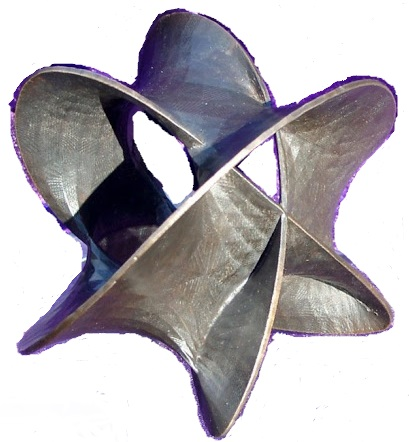
\includegraphics[width=2cm]{K3}};
  \draw[dashed, color=gray] (0,0,0) -- (0,0,4);
    \draw[dashed, color=gray] (0,0,0) -- (0,4,0);
    \draw[dashed, color=gray] (0,0,0) -- (4,0,0);
    \draw (0,4,0) -- (0,0,4);
    \draw (0,4,0) -- (4,0,0);
    \draw (4,0,0) -- (0,0,4);

	\end{tikzpicture}
\end{center}

\begin{comment}
\begin{center}
 \begin{tikzpicture}
   \node[opacity=0.3] (img1) at (0.8453,0.8453,0.8453) {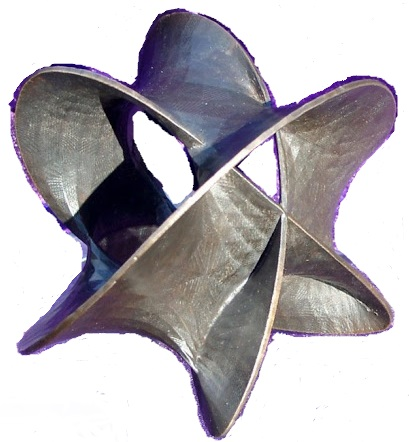
\includegraphics[width=2cm]{K3}};
  \draw[dashed, color=gray] (0,0,0) -- (0,0,4);
    \draw[dashed, color=gray] (0,0,0) -- (0,4,0);
    \draw[dashed, color=gray] (0,0,0) -- (4,0,0);
    \draw (0,4,0) -- (0,0,4);
    \draw (0,4,0) -- (4,0,0);
    \draw (4,0,0) -- (0,0,4);

    \filldraw[gray] (0.8453,0.8453,0) -- (0.8453,0.8453,0.8453) -- (0.8453,0,0.8453) -- (0.8453,0,0) -- cycle;
 %   \draw (0.8453,0.8453,0.8453) -- (0.8453,0,0.8453);

	\end{tikzpicture}
\end{center}
\end{comment}

\subsection{Тропический миррор (анонс)}

В А-модели задача формулируется так: сколько определённых кривых\que{картинка?} пройдёт через отмеченные циклы\que{здесь тонкость: нужно переопределить понятие цикла}.

$$\text{A-сторона:} \hskip 20 pt H = \vec p \cdot \vec n + \sum\limits_{\delta} V_{\delta}$$
$$\text{B-сторона:} \hskip 20 pt H = \frac{\p}{\p \vec x} \frac{\p}{\p \vec y} + e^{\vec \delta \vec y}$$

Видно, что А- и B-стороны связаны просто-напросто Фурье-преобразованием. На B-стороне получается теория поля; так получающаяся теория поля называется теорией Бершадского---Чекотти---Огури---Вафы (только они писали для обычной комплексной структуры, а надо для деформированной суперпотенциалом).

\section{Связь суперконформной теории поля и теории Саито}
\subsection{Строим основной объект, деформируем дифференциал Бельтрами}

Introduce several moduli spaces:

$$\mathcal{M}_g = \{\text{все дифференциалы Бельтрами}\} / \{\text{диффеоморфизмы}\}$$

$$\mathcal{M}_{g,n} = \{\text{все дифференциалы Бельтрами}\} / \{\text{диффеоморфизмы, обращающиеся в ноль}\}$$

$$\mathcal{\hat M}_{g,n} = \{\text{все дифференциалы Бельтрами}\} / \{\text{диффеоморфизмы, имеющие нулевой росток}\}$$

И объявим главным объектом рассмотрения т.н. <<основной объект>> $I$:

\be I^{(k,l)} = \langle  V_1 (z_1) ... V_n (z_n) \int\limits_{\Sigma} G \cdot \mu^{(1)} ... \int\limits_{\Sigma} G \cdot \mu^{(k)} \int\limits_{\Sigma} \bar G \cdot \bar \mu^{(1)} \int\limits_{\Sigma} \bar G \cdot \bar \mu^{(l)}                          \rangle   \ee

Теперь продеформируем $\mu$ векторным полем: $\mu \to \mu + \bar\p v$ ($v$ не может иметь нули более чем первого порядка, но хотя бы один ноль первого порядка имеет), получим выражение вида $$\int\limits_{\Sigma} \bar\p (Gv)$$
и произведём интегрирование по частям в $\delta I$.


На пространстве вертексных операторов действует $Q_{\varepsilon} = Q + \varepsilon G_0$. Возьмём два каких-то вертексных оператора и потребуем, чтобы $$V_1 - \varepsilon \tilde V_1 = Q_{\varepsilon} (...).$$ Тогда для основного объекта верно $$I(V_1, ...) \sim c_1 (\mathcal{L}_1) \wedge I(\tilde V_1, ...)$$

Подействуем: $$(d + \varepsilon \iota_v) A = F + \varepsilon,$$

$F$ и $\varepsilon$ не просто замкнуты по отдельности, но ещё и их сумма точна. Поэтому $\varepsilon$ представляется первым классом Черна.

Формула Картана и соотношение между тензором энергии-импульса $T$, его суперпартнёром $G$ и дифференциалом де Рама $Q$ невероятно похожи:
$$\mathcal{L}_v  = \{d, \iota_v\}$$
$$T = \{Q, G\}$$

Поэтому эти матфизические величины можно интерпретировать так: $T$ --- то, что представляет диффеоморфизмы, $Q$ --- то, что представляет дифференциал де Рама, $G$ --- то, что представляет подстановку векторного поля.

\subsection{Saito theory}

The theory of Kyoji Saito answers the question of how to construct the connection in the cohomology of $Q_{\varepsilon}$.

Why do we need it? Because this connection together with the Gauss---Manin connection form the flat sheaf and provide us the WDVV equation.


\subsubsection{Изложение хронологическое}

Сам Саито занимался, как известно, теорией особенностей и начал с изучения таких интегралов: $$\int \frac{\Omega}{W - t_0},$$ а также их производных по $t_0$. Он заметил, что удобно ввести величину $\varepsilon := \Big(\frac{\p}{\p t_0} \Big)^{-1}$. Потом Варченко указал ему, что его интегралы --- то же, что интегралы вида $$\int\limits_{\Gamma} e^{\frac{W}{\varepsilon}} \Omega.$$

Некоторые из них оказываются нулями. При каких условиях?

Рассмотрим самый простой --- одномерный случай, $\Omega = P dx = d\tilde P$. Получаем $$- \int e^{\frac{W}{\varepsilon}} d\tilde P = \int d \Big( e^{\frac{W}{\varepsilon}} \Big) \tilde P = \int \frac{dW}{\varepsilon} e^{\frac{W}{\varepsilon}} \tilde P,$$ $$\int (d + \frac{dW}{\varepsilon}) \tilde P e^{\frac{W}{\varepsilon}} = 0$$ $$\int (\varepsilon d + dW) \tilde P e^{\frac{W}{\varepsilon}} = 0$$

Чтобы искомая связность $\Omega = d\tilde P$ была плоская, надо потребовать $(\varepsilon d + dW) \tilde P = 0$.

Порассматриваем какие-нибудь простейшие суперпотенциалы. Пусть, например, $W = x^2$. Методом неопределённых коэффициентов найдём связность $\tilde P$: $$(\varepsilon d + 2x) (\alpha_0 + \alpha_1 x + \alpha_2 x^2 + \alpha_3 x^3 + ...) = 0$$ $$\Big(\varepsilon \alpha_1 + 2 \varepsilon \alpha_2 x + 3 \varepsilon \alpha_3 x^2 + ...\Big) + \Big(2 \alpha_0 x + 2 \alpha_1 x^2 + 2 \alpha_2 x^3 + ...\Big) = 0,$$ откуда можно вытащить такую череду равенств: $$\varepsilon \alpha_1 = 0$$
$$2 \varepsilon \alpha_2 + 2 \alpha_0 = 0$$
$$3 \varepsilon \alpha_3 + 2 \alpha_1 = 0$$
$$4 \varepsilon \alpha_4 + 2 \alpha_2 = 0$$
 и так далее. Из неё вполне видно, что все нечётные $\alpha_i$ равны нулю, а все чётные удовлетворяют равенству $$\alpha_{2n} = \frac{(-1)^n}{\varepsilon^n n!} \alpha_0.$$ Поэтому плоская связность для такого суперпотенциала равна дифференциалу де Рама от следующего выражения:

 $$\tilde P = \alpha_0 - \frac{1}{\varepsilon 1!} \alpha_0 x^2 + \frac{1}{\varepsilon^2 2!} \alpha_0 x^4 + ...$$

 Приравняем к единице несущественный общий множитель. Возьмём дифференциал и получим наконец плоскую связность для суперпотенциала $W = x^2$:

$$\Omega = d\tilde P = d \sum\limits_n \frac{(-1)^n}{\varepsilon^n n!} x^{2n} = \boxed{\sum\limits_n \frac{(-1)^n}{\varepsilon^n (n-1)!} x^{2n-1} }$$

 (множитель $2$ опущен как общий).

Аналогично можно рассмотреть $W = x^3$.





$\varepsilon$ генерирует $\psi$-классы Мориты---Мамфорда\que{Раскрыть.}.


\subsubsection{Изложение теоретико-полевое}

$$S = \int \Big( \p X \bar \p \bar X + \bar \pi \p \bar \psi + \pi \bar \p \psi  \Big)$$

$$G = \pi \p \bar X$$
$$J = \psi \p X$$

Как устроены поля конформной размерности 0? Вот так: $F(X, \bar X, \psi, \bar \psi)$.

Однако можно сделать замену вида $\rho = \psi + \bar \psi$, $\theta = (\psi - \bar \psi) g$. Тогда внезапно оказывается, что $F(X, \bar X, \rho^{\bar i}, \theta_i)$ --- не что иное, как поливекторные поля со значениями в $(0,\bullet)$-формах.

$$QP = \rho \frac{\p}{\p \bar X} P = \bar \p^{t} P$$

$$G_0 - \bar G_0 = \frac{\p}{\p \theta_i} \frac{\p}{\p X^i} = \Delta_{BV}$$

Это всё было при $W=0$. Если <<включить>> суперпотенциал, ток изменится на такой: $$J = \psi \p X + W' \pi$$ а дифференциал превратится в такой:

$$Q + \varepsilon G_0 = \bar\p + \varepsilon \Delta_{BV} + \frac{\p W}{\p X^i} \frac{\p}{\p \theta_i},$$

$\bar\p$ --- дифференциал свободной теории, $\varepsilon \Delta_{BV}$ --- эквивариантная добавка, $\frac{\p W}{\p X^i} \frac{\p}{\p \theta_i}$ --- вызванное наличием суперпотенциала возмущение.

\section{Topological quantum mechanics}
\subsection{$A_{\infty}-$structure and one the contexts of its appearance}

Попробуем спасти идею функционального интеграла. Исторически он регуляризовывался введением решётки. Однако, как заметил Колмогоров в 50-е гг.,  на коцепях нет ассоциативного умножения\que{почему?}. На дифференциальных формах есть ассоциативное умножение, а вот на симплициальной реализации того же самого --- как оказалось, нет. Однако там есть почти ассоциативное умножение --- $A_{\infty}$-структура.

For example, $m_2$ is associative up to the higher operations:

\begin{center}
 \begin{tikzpicture}

%  \draw[->, color=gray, thick] (0,0) -- (10,0) node[right] {$z_T$};
%  \draw[->, color=gray, thick] (0,0) -- (0,6) node[above] {$w_T$};
  \draw[very thick] (1.5,5) -- (2,4);
    \draw[very thick] (1.5,3) -- (2,4);
    \filldraw [black] (2,4) circle (2pt);
        \filldraw [black] (4,3) circle (2pt);
            \draw[very thick] (2,4) -- (4,3);
            \draw[very thick] (4,3) -- (3.5,2);
            \draw[very thick] (4,3) -- (4.5,2);
  \draw (2,4) node[above=1pt, right=1pt] {$m_2$};
  \draw (4,3) node[above=1pt, right=1pt] {$m_2$};

  \draw (1.5,3) node[below=1pt] {$1$};
  \draw (3.5,2) node[below=1pt] {$2$};
  \draw (4.5,2) node[below=1pt] {$3$};

    \draw (6,3.5) node {$-$};

  \draw[very thick] (7.5,2) -- (8,3);
    \draw[very thick] (8.5,2) -- (8,3);
    \filldraw [black] (8,3) circle (2pt);
        \filldraw [black] (9,4) circle (2pt);
            \draw[very thick] (8,3) -- (9,4);
            \draw[very thick] (9,4) -- (9.5,3);
            \draw[very thick] (9,4) -- (9.5,5);
  \draw (8,3) node[above=1pt, left=1pt] {$m_2$};
  \draw (9,4) node[above=1pt, left=1pt] {$m_2$};

 \draw (7.5,2) node[below=1pt] {$1$};
  \draw (8.5,2) node[below=1pt] {$2$};
 \draw (9.5,3) node[below=1pt] {$3$};

    \draw (11,3.5) node {$=$};

    \draw (12,3.5) node {$d(m_3)$};

	\end{tikzpicture}
\end{center}


There are $n-$ary operations: $d, m_2, m_3, m_4, ...$. And this is how can they be depicted:

\begin{center}
 \begin{tikzpicture}


  \draw (0,2.5) -- (0,2) -- (0.5,2) -- (0.5,2.5) -- cycle;
  \draw (-1,2.25) -- (0,2.25);
  \draw (0.5,2.25) -- (1.5,2.25);
    \draw (2,2.25) node[right=1pt] {$d$};

    \draw (0,1.5) -- (0,1) -- (0.5,1) -- (0.5,1.5) -- cycle;
  \draw (-1,1.25) -- (0,1.25);
    \draw (-1,1.125) -- (0,1.125);
      \draw (-1,1.375) -- (0,1.375);
  \draw (0.5,1.25) -- (1.5,1.25);
      \draw (2,1.125) node[right=1pt] {$m_3$};

  \draw (0,0.5) -- (0,0) -- (0.5,0) -- (0.5,0.5) -- cycle;
  \draw (-1,0.167) -- (0,0.167);
    \draw (-1,0.33) -- (0,0.33);
  \draw (0.5,0.25) -- (1.5,0.25);
      \draw (2,0.25) node[right=1pt] {$m_2$};

	\end{tikzpicture}
\end{center}

The pack of operations $(d, m_2, m_3, ...)$ admitting the (super-)Leibnitz rule is called $A_{\infty}$-structure.

In string theory these diagrams will look like

\begin{center}
\begin{tikzpicture}


%\fill[cyan!10] (4,0) rectangle (0,3);

%\fill[cyan!10] (0.11,3.4) arc (-175:-5:1.9cm and 0.6cm) -- (3.89,2.45) -- (0.11,2.45) -- cycle;
%\fill[cyan!10] (3.89,-0.4) arc (5:175:1.9cm and 0.6cm) -- (0.11,0.55) -- (3.89,0.55) -- cycle;

	\draw[thick] (4,1.5) ellipse (0.166 and 0.5);% right ellipse
	\draw[thick] (0,3) ellipse (0.166 and 0.5);% left top ellipse
	\draw[thick] (0,0) ellipse (0.166 and 0.5);% left bottom ellipse
\draw[thick] (-0.1,0.4) arc (-45:45:1cm and 1.55cm); % left arc
\draw[thick] (4,1) arc (95:178:4.2cm and 1.2cm); % bottom arc
\draw[thick] (0.15,3.2) arc (-180:-95:4.2cm and 1.2cm); % top arc
      \draw (2,-1) node[below=1pt] {$m_2$};

	\draw[thick] (7,1.5) ellipse (0.166 and 0.5);% right ellipse
	\draw[thick] (11,1.5) ellipse (0.166 and 0.5);% left top ellipse
\draw[thick] (7,1) -- (11,1);
\draw[thick] (7,2) -- (11,2);
      \draw (9,-1) node[below=1pt] {$d$ (она же $m_1$)};

\end{tikzpicture}
\end{center}


\subsection{Renormalization in topological quantum mechanics}


Общепринятым способом избегания УФ расходимостей является введение параметра обрезания:
$$\int d^N p \longrightarrow \int\limits_0^{\Lambda} d^N p$$

Способ ввести параметр обрезания <<в лоб>> в топологической квантовой механике --- ограничиться на формы $\Omega_X^{\bullet \Lambda}$ --- на формы, у которых импульсы, получающиеся после преобразования Фурье функции, стоящей перед $dx^1 \wedge ... \wedge dx^n$, ограничены по модулю числом $\Lambda$: $$\Omega_X^{\bullet \Lambda} := \Omega_X^{\bullet}\Big|_{|\vec p| < \Lambda}, \hskip 20 pt \Omega_X^{\bullet} \longrightarrow \Omega_X^{\bullet \Lambda}.$$ Но на $\Omega_X^{\bullet \Lambda}$ уже нет структуры dg-алгебры\que{кстати, почему?}. Проблема.

Необходим более умный способ перенормировки. (Где здесь вообще может возникнуть расходимость? Она может возникнуть, если вершины сталкиваются. Коррелятор в таком случае может быть не определён, а вклад пропагатора будет стремиться к тождественному оператору.)

Предложение заключается в том, чтобы перейти к швингеровскому представлению пропагатора и затем перенормировать <<время>>:

$$\int\limits_{\tau_{\text{ш}}}^{\infty} d\tau e^{-\tau \Delta} = [\tau' = \tau - \tau_{\text{ш}}] = \int\limits_0^{\infty} d\tau' e^{-(\tau' + \tau_{\text{ш}}) \Delta} = e^{-\tau_{\text{ш}} \Delta} \int\limits_0^{\infty} d\tau' e^{-\tau' \Delta} = e^{-\tau_{\text{ш}} \Delta} \frac{1}{\Delta},$$ т.е. перенормированный пропагатор вот каков:

$$\frac{1}{\Delta_{\text{ren}}} = e^{-\tau_{\text{ш}} \Delta} \frac{1}{\Delta}.$$

Let us mark this way renormalized propagator with the letter <<s>> (Schwinger representation):


\begin{center}
 \begin{tikzpicture}

\draw (-1,0) -- (1,0);
   \filldraw[color=white, rounded corners] (-0.5,-0.25) rectangle (0.5,0.25);
  \draw[rounded corners] (-0.5,-0.25) rectangle (0.5,0.25);
\node at (0,0) {\text{s}};

	\end{tikzpicture}
\end{center}

Впоследствии мы будем делать утверждения вида <<такой-то пропагатор чему-то равен>>. В целях удобства обсуждения договоримся опускать в них множитель $1/\Delta$. В рамках этой договорённости у нас получилось, что

\begin{center}
 \begin{tikzpicture}

\draw (-1,0) -- (1,0);
   \filldraw[color=white, rounded corners] (-0.5,-0.25) rectangle (0.5,0.25);
  \draw[rounded corners] (-0.5,-0.25) rectangle (0.5,0.25);
\node at (0,0) {\text{ш}};

    \draw (1.5,0) node {$=$};

    \draw (2.5,0) node {$e^{-\tau_{\text{s}} \Delta},$};

\draw (3.5,0) -- (5.5,0);
    \draw (6,0) node {$=$};

    \draw (6.5,0) node {$1$};
	\end{tikzpicture}
\end{center}

An example of this way renormalized diagram:

\begin{center}
 \begin{tikzpicture}



\draw (-1,0) -- (1,0);
%\draw (-0.2,-0.25) -- (-0.2,0.25) -- (0.2,0.25) -- (0.2,-0.25) -- cycle;

\draw (1,0) -- (3,1);
\draw (1,0) -- (3,-1);

\draw (-1,0) -- (-3,1);
\draw (-1,0) -- (-3,-1);

%\tikzset{anchor=west}

\filldraw[color=white, rounded corners] (-0.5,-0.25) rectangle (0.5,0.25);
\draw[rounded corners] (-0.5,-0.25) rectangle (0.5,0.25);
 \draw (0,0) node {\text{s}};

 \filldraw[color=white, rotate around={26.57:(1,0)}, rounded corners] (1.618,-0.25) rectangle (2.618,0.25);
  \draw[rotate around={26.57:(1,0)},rounded corners] (1.618,-0.25) rectangle (2.618,0.25);

   \filldraw[color=white, rotate around={-26.57:(1,0)}, rounded corners] (1.618,-0.25) rectangle (2.618,0.25);
  \draw[rotate around={-26.57:(1,0)},rounded corners] (1.618,-0.25) rectangle (2.618,0.25);

   \filldraw[color=white, rotate around={26.57:(-1,0)}, rounded corners] (-1.618,-0.25) rectangle (-2.618,0.25);
  \draw[rotate around={26.57:(-1,0)},rounded corners] (-1.618,-0.25) rectangle (-2.618,0.25);

   \filldraw[color=white, rotate around={-26.57:(-1,0)}, rounded corners] (-1.618,-0.25) rectangle (-2.618,0.25);
  \draw[rotate around={-26.57:(-1,0)},rounded corners] (-1.618,-0.25) rectangle (-2.618,0.25);



%\draw[rotate=0] (2.2,0) node[rotate around={26.57:(1,0)}] {\text{ш}};
%\node[rotate around={26.57:(1,0)}] at (2,0.5) {\text{ш}};

\node[rotate=26.57] at (2,0.5) {\text{s}};
\node[rotate=-26.57] at (2,-0.5) {\text{s}};

\node[rotate=-26.57] at (-2,0.5) {\text{s}};
\node[rotate=26.57] at (-2,-0.5) {\text{s}};

%\node[draw, rotate around={60:(-1,0)}]


%\foreach \x/\y in {0.8944/0, 1.7889/0, 2.6833/0, 3.5777/0}
 %   \draw[rotate=26.57,dashed,thick,color=cyan] (\x,\y) ellipse (0.1cm and 0.3cm);

%\draw[rounded corners,red,rotate around={30:(-1,0.5)}] (-3.5,0) rectangle (-0.5,2);


	\end{tikzpicture}
\end{center}

Jokingly we will call such Schwinger propagators <<resistors>>.

Если отнести деформации пропагатора к вершинам и воспринимать их уже как деформации операторов, стоящих в вершинах, то получится как раз $A_{\infty}$-структура.


\subsection{Об аксиальной аномалии}


Далее, есть такой хорошо известный математический факт --- что лапласиан есть суперкоммутатор дифференциала де Рама $d$ и сопряжённого к нему по Ходжу $d^*$. Т.е. $$e^{-\tau_{\text{ш}} \Delta} = e^{-\tau_{\text{ш}} \{ d, d^* \} }$$

Обсудим аномальный распад $\pi^0 \to 2\gamma$.

$$\psi_L \to e^{i\alpha} \psi_L $$

$$\psi_R \to e^{-i\alpha} \psi_R $$

$$\operatorname{Tr}_{\text{Spin}} \gamma^5 e^{-\beta \slashed{D}^2_A} = \operatorname{Str} e^{-\beta \slashed{D}^2_A}$$

Эйлерова характеристика:

$$\chi = \operatorname{Str}_{\Omega^{\bullet}} e^{-\tau_{\text{ш}} \{ d, d^* \}  } $$

Арифметический род:

$$H\chi = \operatorname{Str}_{\Omega^{0,\bullet}} e^{-\tau_{\text{ш}} \{ \bar \p, \bar \p^* \}  } $$

\subsection{Как вычислять амплитуды}

Вот BV-регуляризация по Костелло:

\begin{center}
 \begin{tikzpicture}

\draw (-1,0) -- (1,0);

    \draw (1.5,0) node {=};

    \draw (3,0) node {$e^{-\tau_{\text{ш}} \{Q,G\}}$};

   \filldraw[color=white, rounded corners] (-0.5,-0.25) rectangle (0.5,0.25);
  \draw[rounded corners] (-0.5,-0.25) rectangle (0.5,0.25);
\node at (0,0) {\text{ш}};

	\end{tikzpicture}
\end{center}

Рецепт вычисления амплитуд: необходимо проинтегрировать по всем внутренним линиям, а входы и выходы замкнуть на когомологии. Если подстановка резистора (отличие резистора от его отсутствия) --- $Q$-точная вещь:

\begin{center}
 \begin{tikzpicture}

\draw (-1,0) -- (1,0);


   \filldraw[color=white, rounded corners] (-0.5,-0.25) rectangle (0.5,0.25);
  \draw[rounded corners] (-0.5,-0.25) rectangle (0.5,0.25);
\node at (0,0) {\text{ш}};

    \draw (1.5,0) node {$-$};

        \draw (2,0) node {$1$};

    \draw (2.5,0) node {$=$};

    \draw (3.25,0) node {$Q(..),$};

	\end{tikzpicture}
\end{center}

то ответ не будет зависеть от величины швингеровского обрезания. Нас интересует именно $Q$-точный случай как самый красивый и реалистичный, ибо если на графах существует суперпартнёр тензора энергии-импульса $G$, то подстановка резистора $Q$-точна.


\begin{center}
 \begin{tikzpicture}

\filldraw [black] (0,0) circle (2pt);
\draw (0,0) node[below=1pt] {$0$};

\draw (0,0) -- (1,0);

\filldraw [black] (1,0) circle (2pt);
\draw (1,0) node[below=1pt] {$\tau_{\text{ш}}$};

\draw (3.5,0) node {$= \{Q, \int\limits_0^{\tau_{\text{ш}}} e^{-\tau \{ Q,G\} } G d\tau \}$};


	\end{tikzpicture}
\end{center}

Зачем вводить теорию струн in order to avoid divergences, когда это можно сделать проще с помощью топологической квантовой механики?

\subsection{Постоянная Планка --- скрытое число петель (внутренних и внешних)}

\begin{center}

Фейнман: $e^{\frac{1}{\hbar} S}$

Костелло---Швингер---Цвибах: $e^{\frac{1}{\hbar} S(\hbar)}$

\end{center}

Гений Баталина(?) состоял в том, чтобы написать действие, зависящее от постоянной Планка, а не как у Фейнмана\que{Раскрыть эту мысль и раскрыть мысль, вынесенную в заголовок.}.

Ещё раз: после перехода к дискретному пространству теория струн становится теорией частиц, в которой очень много вершин и пропагаторов между ними. После перехода к дискретному пространству теория струн --- частный случай описанной выше конструкции. Это придумал Цвибах, но побоялся включить в свою книжку по теории струн.

\begin{comment}
\section{Способ разрешения парадокса Хокинга}

\begin{center}
\begin{tikzpicture}

\tikzset{snake it/.style={decorate, decoration=snake}}

%  \path [draw=blue,snake it]
 %   (-4,0) -- (-2,0) -- (2,0) -- (4,0);
%  \draw[draw=blue, snake it] (2,0) arc (0:180:2cm);

\draw (-3.25,3) node[above=1pt] {$N \to \infty$};

\draw[thick] (-3,3) -- (-3,-3);
\draw[thick] (-3.125,3) -- (-3.125,-3);
\draw[thick] (-3.25,3) -- (-3.25,-3);
\draw[thick] (-3.375,3) -- (-3.375,-3);
\draw[thick] (-3.5,3) -- (-3.5,-3);

\draw[thick,snake it] (-3,0) -- (1,0);
\draw (-1,0) node[above=1pt] {\text{струна}};

\draw (-3.25,-3) node[below=1pt] {\text{D-брана}};

\end{tikzpicture}
\end{center}

Хокинг изучал чёрные дыры, далёкие от критических ($M \gg Q$). А в случае чёрных дыр, близких к критическим ($M \approx Q$), площадь горизонта чёрной дыры совпадает с числом степеней свободы такой пачки D-бран.


\end{comment}

\section{Концевич и теория деформаций}

\begin{center}
 \begin{tikzpicture}

\tikzset{cross/.style={cross out, draw=black, minimum size=2*(#1-\pgflinewidth), inner sep=0pt, outer sep=0pt},
%default radius will be 1pt.
cross/.default={6pt}}

\foreach \x/\y/\z/\a in {-1.329/-1.495/1.329/1.495, -1.516/-1.305/1.118/1.658, -1.118/-1.658/1.516/1.305, -1.678/-1.088/0.884/1.794, -0.884/-1.794/1.678/1.088, -1.814/-0.841/0.623/1.901, -0.623/-1.901/1.814/0.841, -1.920/-0.560/0.331/1.972, -0.331/-1.972/1.920/0.560, -1.986/-0.234/0/2, 0/-2/1.986/0.234, -1.994/0.157/-0.390/1.962, 0.390/-1.962/1.994/-0.157, -1.878/0.687/-0.902/1.785, 0.902/-1.785/1.878/-0.687}
    \draw[ultra thin,color=black!10] (\x,\y) -- (\z,\a);



\draw[thick] (0,0) circle (2);

\filldraw [black] (-0.5,1) circle (2pt);
\filldraw [black] (-0.2,-1.5) circle (2pt);
\filldraw [black] (1,-0.5) circle (2pt);

\foreach \x/\y in {2/0, -0.329/-1.973, -1.638/-1.147, -1.789/0.894}
  \draw[ultra thick] (\x,\y) node[cross] {};

%now let's draw the exit
\tikzstyle{vecArrow} = [thick, decoration={markings,mark=at position
   1 with {\arrow[semithick]{open triangle 60}}},
   double distance=1.4pt, shorten >= 5.5pt,
   preaction = {decorate},
   postaction = {draw,line width=1.4pt, white,shorten >= 4.5pt}]
\tikzstyle{innerWhite} = [semithick, white,line width=1.4pt, shorten >= 4.5pt]

  \draw[vecArrow] (1.372,0.823) to (2.058,1.235);
  \draw[innerWhite] (1.372,0.823) to (2.058,1.235);

  \draw (1.715,1.4) node[right=1pt] {\text{выход}};


%\filldraw [black] (0,0) circle (2pt);
%\draw (0,0) node[below=1pt] {$0$};

%\filldraw [black] (1,0) circle (2pt);
%\draw (1,0) node[below=1pt] {$\tau_{\text{ш}}$};


	\end{tikzpicture}
\end{center}

Есть три взгляда на то, что такое локальная наблюдаемая.

Согласно Фейнману, локальная наблюдаемая --- некоторая функция от значений полей и их производных в точке $x_0$.

Согласно Полякову, локальная наблюдаемая --- некоторый предел решёточных статсумм.

Согласно Сигалу, локальная наблюдаемая получается стягиванием окружности в точку:

\begin{center}
\begin{tikzpicture}


\fill[cyan!10] (4,0) rectangle (0,3);

\fill[cyan!10] (0.11,3.4) arc (-175:-5:1.9cm and 0.6cm) -- (3.89,2.45) -- (0.11,2.45) -- cycle;
\fill[cyan!10] (3.89,-0.4) arc (5:175:1.9cm and 0.6cm) -- (0.11,0.55) -- (3.89,0.55) -- cycle;

	\draw[thick,dashed,fill=white] (4,3) ellipse (0.166 and 0.5);% right top ellipse
	\draw[thick,fill=white] (0,3) ellipse (0.166 and 0.5);% left top ellipse
	\draw[thick,fill=white] (4,0) ellipse (0.166 and 0.5);% right bottom ellipse
	\draw[thick,fill=white] (0,0) ellipse (0.166 and 0.5);% left bottom ellipse
\draw[thick,fill=white] (-0.1,0.4) arc (-45:45:1cm and 1.55cm); % left arc
\draw[thick,fill=white] (3.89,-0.4) arc (5:175:1.9cm and 0.6cm); % bottom arc
\draw[thick,fill=white] (4.1,2.6) arc (135:225:1cm and 1.55cm); % right arc
\draw[thick,fill=white] (0.11,3.4) arc (-175:-5:1.9cm and 0.6cm); % top arc


%\draw[thick] (3.26,3.44) -- (3.76,4.64);
%\draw[thick] (4,2.5) -- (4.5,3.7);

\draw[thick] (4,3.5) -- (7,3);
\draw[thick] (4,2.5) -- (7,3);

	\draw[thick,dashed,fill=white] (4.6,3) ellipse (0.133 and 0.4);
	\draw[thick,dashed,fill=white] (5.2,3) ellipse (0.100 and 0.3);
	\draw[thick,dashed,fill=white] (5.8,3) ellipse (0.066 and 0.2);
	\draw[thick,dashed,fill=white] (6.4,3) ellipse (0.033 and 0.1);


%	\draw[thick,fill=white, dashed] (4,3) ellipse (0.166 and 0.5);

\end{tikzpicture}
\end{center}



\footnotesize{}

Если угодно, здесь возможна такая аналогия. <<Поляковский>> взгляд на число Эйлера --- число Эйлера $e$ есть предел следующей последовательности: $$e = \lim\limits_{n \to \infty} \Big(1 + \frac{1}{n} \Big)^n$$

<<Сигаловский>> же взгляд --- решите уравнение $f'(x) = f(x)$ как хотите (рецепт не предоставляется), и когда вы его решите (любым из способов), окажется, что $$e = \frac{f(1)}{f(0)}.$$

\normalsize{}

\subsection{Пока не пережали}

Пока не пережали, была сфера. Все точки --- $\Phi$, и только одна --- $\tilde \Phi$:

\begin{center}
 \begin{tikzpicture}

\tikzset{cross/.style={cross out, draw=black, minimum size=2*(#1-\pgflinewidth), inner sep=0pt, outer sep=0pt},
%default radius will be 1pt.
cross/.default={6pt}}

%\foreach \x/\y/\z/\a in {-1.329/-1.495/1.329/1.495, -1.516/-1.305/1.118/1.658, -1.118/-1.658/1.516/1.305, -1.678/-1.088/0.884/1.794, -0.884/-1.794/1.678/1.088, -1.814/-0.841/0.623/1.901, -0.623/-1.901/1.814/0.841, -1.920/-0.560/0.331/1.972, -0.331/-1.972/1.920/0.560, -1.986/-0.234/0/2, 0/-2/1.986/0.234, -1.994/0.157/-0.390/1.962, 0.390/-1.962/1.994/-0.157, -1.878/0.687/-0.902/1.785, 0.902/-1.785/1.878/-0.687}
 %   \draw[ultra thin,color=black!10] (\x,\y) -- (\z,\a);



\draw[thick] (0,0) circle (2);

\foreach \x/\y in {0.625/0.188, -0.357/0.893, -1.324/0.210, -0.5/-0.5, 1.321/-0.348, -0.964/-1.317, 0.985/1.074, 0.741/-1.535}
\filldraw [black] (\x,\y) circle (2pt);

\draw[thick] (0.8,0.288) -- (4,1);

\draw (4,1) node[right=1pt] {$\tilde \Phi$};


%\foreach \x/\y in {-0.329/-1.973, -1.789/0.894}
 % \draw[ultra thick] (\x,\y) node[cross] {};

%\tikzstyle{vecArrow} = [thick, decoration={markings,mark=at position
 %  1 with {\arrow[semithick]{open triangle 60}}},
 %  double distance=1.4pt, shorten >= 5.5pt,
%   preaction = {decorate},
 %  postaction = {draw,line width=1.4pt, white,shorten >= 4.5pt}]
%\tikzstyle{innerWhite} = [semithick, white,line width=1.4pt, shorten >= 4.5pt]

%% \draw[vecArrow] (1.372,0.823) to (2.058,1.235);
  %\draw[innerWhite] (1.372,0.823) to (2.058,1.235);


%  \draw (-2.1,0.994) node[above=1pt] {$f_1 (x)$};
 %   \draw (-0.329,-2.073) node[below=1pt] {$f_2 (x)$};

%  \draw (1.715,1.4) node[right=1pt] {$\delta(x-x_0)$};

%\draw (3,0) node {\Huge{=}};

%\draw (5,0) node {$(f_1 \cdot f_2) (x_0)$};

	\end{tikzpicture}
\end{center}

После того, как пережали,


\begin{center}
 \begin{tikzpicture}

\tikzset{cross/.style={cross out, draw=black, minimum size=2*(#1-\pgflinewidth), inner sep=0pt, outer sep=0pt},
%default radius will be 1pt.
cross/.default={6pt}}

\draw[thick] (-4,0) circle (2);

\foreach \x/\y in {-4.357/0.893, -5.324/0.210, -4.5/-0.5, -4.964/-1.317}
\filldraw [black] (\x,\y) circle (2pt);

\draw[thick] (4,0) circle (2);

\foreach \x/\y in {4.625/0.188, 5.321/-0.348, 4.985/1.074, 4.741/-1.535}
\filldraw [black] (\x,\y) circle (2pt);

\filldraw [white] (-2.108,0.174) rectangle (2.108,-0.174);

\draw[thick] (-2.008,0.174) -- (2.008,0.174);
\draw[thick] (-2.008,-0.174) -- (2.008,-0.174);


\draw[thick] (4.8,0.288) -- (8,1);

\draw (8,1) node[right=1pt] {$\tilde \Phi$};


	\end{tikzpicture}
\end{center}

левая половина стала для правой наблюдаемой типа $\Phi$ (бесконечно далёкой, похожей на точку). Правая половина стала для левой наблюдаемой типа $\tilde \Phi$ (тоже бесконечно далёкой и похожей на точку).

\subsection{Постановка задачи о деформационном квантовании}

\begin{center}
 \begin{tikzpicture}

\tikzset{cross/.style={cross out, draw=black, minimum size=2*(#1-\pgflinewidth), inner sep=0pt, outer sep=0pt},
%default radius will be 1pt.
cross/.default={6pt}}

\foreach \x/\y/\z/\a in {-1.329/-1.495/1.329/1.495, -1.516/-1.305/1.118/1.658, -1.118/-1.658/1.516/1.305, -1.678/-1.088/0.884/1.794, -0.884/-1.794/1.678/1.088, -1.814/-0.841/0.623/1.901, -0.623/-1.901/1.814/0.841, -1.920/-0.560/0.331/1.972, -0.331/-1.972/1.920/0.560, -1.986/-0.234/0/2, 0/-2/1.986/0.234, -1.994/0.157/-0.390/1.962, 0.390/-1.962/1.994/-0.157, -1.878/0.687/-0.902/1.785, 0.902/-1.785/1.878/-0.687}
    \draw[ultra thin,color=black!10] (\x,\y) -- (\z,\a);



\draw[thick] (0,0) circle (2);


\foreach \x/\y in {-0.329/-1.973, -1.789/0.894}
  \draw[ultra thick] (\x,\y) node[cross] {};

%now let's draw the exit
\tikzstyle{vecArrow} = [thick, decoration={markings,mark=at position
   1 with {\arrow[semithick]{open triangle 60}}},
   double distance=1.4pt, shorten >= 5.5pt,
   preaction = {decorate},
   postaction = {draw,line width=1.4pt, white,shorten >= 4.5pt}]
\tikzstyle{innerWhite} = [semithick, white,line width=1.4pt, shorten >= 4.5pt]

  \draw[vecArrow] (1.372,0.823) to (2.058,1.235);
  \draw[innerWhite] (1.372,0.823) to (2.058,1.235);


  \draw (-2.1,0.994) node[above=1pt] {$f_1 (x)$};
    \draw (-0.329,-2.073) node[below=1pt] {$f_2 (x)$};

  \draw (1.715,1.4) node[right=1pt] {$\delta(x-x_0)$};

\draw (3,0) node {\Huge{=}};

\draw (5,0) node {$(f_1 \cdot f_2) (x_0)$};

%\filldraw [black] (0,0) circle (2pt);
%\draw (0,0) node[below=1pt] {$0$};

%\filldraw [black] (1,0) circle (2pt);
%\draw (1,0) node[below=1pt] {$\tau_{\text{ш}}$};


	\end{tikzpicture}
\end{center}

По-видимому, в поисках пертурбативной некоммутативной геометрии Концевич в 1997 поставил задачу деформации коммутативных ассоциативных алгебр в классе ассоциативных. Более точно, он поставил задачу найти такое умножение $m_{\bullet} (f_1, f_2)$, которое бы обладало тремя следующими свойствами:

\begin{enumerate}
  \item $m_0 (f_1, f_2) = f_1 f_2$
  \item $\frac{\partial m}{\partial \hbar}\Bigg|_{\hbar \to 0} = \{ f_1, f_2\}^{\pi} := \pi^{ij} (x) \frac{\p f_1}{\p x^i} \frac{\p f_2}{\p x^j}$
  \item $m_{\bullet}$ ассоциативно (??)
\end{enumerate}

Поначалу казалось, что хорошим кандидатом является скобка Мояла: $$f_1 * f_2 = e^{\hbar \pi^{ij} } f_1 (x) f_2 (y)$$

Однако позже стало понятно, что есть ряд моментов\que{что это за моменты?}, ввиду которых она не годится.


Причина ассоциативности:


\begin{center}
 \begin{tikzpicture}

\tikzset{cross/.style={cross out, draw=black, minimum size=2*(#1-\pgflinewidth), inner sep=0pt, outer sep=0pt},
%default radius will be 1pt.
cross/.default={6pt}}

\foreach \x/\y/\z/\a in {-8.329/-1.495/-5.671/1.495, -8.516/-1.305/-5.882/1.658, -8.118/-1.658/-5.484/1.305, -8.678/-1.088/-6.116/1.794, -7.884/-1.794/-5.322/1.088, -8.814/-0.841/-6.377/1.901, -7.623/-1.901/-5.186/0.841, -8.920/-0.560/-6.669/1.972, -7.331/-1.972/-5.080/0.560, -8.986/-0.234/-7/2, -7/-2/-5.014/0.234, -8.994/0.157/-7.390/1.962, -6.610/-1.962/-5.006/-0.157, -8.878/0.687/-7.902/1.785, -6.098/-1.785/-5.122/-0.687}
    \draw[ultra thin,color=black!10] (\x,\y) -- (\z,\a);


    \foreach \x/\y/\z/\a in {-4.329/-1.495/-1.671/1.495, -4.516/-1.305/-1.882/1.658, -4.118/-1.658/-1.484/1.305, -4.678/-1.088/-2.116/1.794, -3.884/-1.794/-1.322/1.088, -4.814/-0.841/-2.377/1.901, -3.623/-1.901/-1.186/0.841, -4.920/-0.560/-2.669/1.972, -3.331/-1.972/-1.080/0.560, -4.986/-0.234/-3/2, -3/-2/-1.014/0.234, -4.994/0.157/-3.390/1.962, -2.610/-1.962/-1.006/-0.157, -4.878/0.687/-3.902/1.785, -2.098/-1.785/-1.122/-0.687}
    \draw[ultra thin,color=black!10] (\x,\y) -- (\z,\a);

\draw (0.2,0) node {\Huge{=}};

\foreach \x/\y/\z/\a in {1.671/0.505/4.329/3.495, 1.484/0.695/4.118/3.658, 1.882/0.342/4.516/3.305, 1.322/0.912/3.884/3.794, 2.116/0.206/4.678/3.088, 1.186/1.159/3.623/3.901, 2.377/0.099/4.814/2.841, 1.080/1.440/3.331/3.972, 2.669/0.028/4.920/2.560, 1.014/1.766/3/4, 3/0/4.986/2.234, 1.006/2.157/2.610/3.962, 3.390/0.038/4.994/1.843, 1.122/2.687/2.098/3.785, 3.902/0.215/4.878/1.313}
    \draw[ultra thin,color=black!10] (\x,\y) -- (\z,\a);


    \foreach \x/\y/\z/\a in {1.671/-3.495/4.329/-0.505, 1.484/-3.305/4.118/-0.342, 1.882/-3.658/4.516/-0.695, 1.322/-3.088/3.884/-0.206, 2.116/-3.794/4.678/-0.912, 1.186/-2.841/3.623/-0.099, 2.377/-3.901/4.814/-1.159, 1.080/-2.560/3.331/-0.028, 2.669/-3.972/4.920/-1.440, 1.014/-2.234/3/0, 3/-4/4.986/-1.766, 1.006/-1.843/2.610/-0.038, 3.390/-3.962/4.994/-2.157, 1.122/-1.313/2.098/-0.215, 3.902/-3.785/4.878/-2.687}
    \draw[ultra thin,color=black!10] (\x,\y) -- (\z,\a);

\draw[thick] (-7,0) circle (2);
\draw[thick] (-3,0) circle (2);

\draw[thick] (3,2) circle (2);
\draw[thick] (3,-2) circle (2);

%\filldraw [black] (-3.5,1) circle (2pt);
%\filldraw [black] (-3.2,-1.5) circle (2pt);
%\filldraw [black] (-2,-0.5) circle (2pt);

%\filldraw [black] (2.5,1) circle (2pt);
%\filldraw [black] (2.8,-1.5) circle (2pt);
%\filldraw [black] (4,-0.5) circle (2pt);

\foreach \x/\y in {-8.638/-1.147, -8.789/0.894}
  \draw[ultra thick] (\x,\y) node[cross] {};

    \draw (-8.789,0.994) node[above=1pt] {$f_1$};
        \draw (-8.638,-1.247) node[below=1pt] {$f_2$};

  \foreach \x/\y in {-1/0}
  \draw[ultra thick] (\x,\y) node[cross] {};

          \draw (-1,-0.1) node[right=1pt] {$f_3$};

  \foreach \x/\y in {1.211/2.894}
  \draw[ultra thick] (\x,\y) node[cross] {};

      \draw (1.211,2.994) node[above=1pt] {$f_1$};

  \foreach \x/\y in {5/-2, 1.362/-3.147}
  \draw[ultra thick] (\x,\y) node[cross] {};

          \draw (1.362,-3.247) node[below=1pt] {$f_2$};

                    \draw (5,-2.1) node[right=1pt] {$f_3$};

%now let's draw the exit
\tikzstyle{vecArrow} = [thick, decoration={markings,mark=at position
   1 with {\arrow[semithick]{open triangle 60}}},
   double distance=1.4pt, shorten >= 5.5pt,
   preaction = {decorate},
   postaction = {draw,line width=1.4pt, white,shorten >= 4.5pt}]
\tikzstyle{innerWhite} = [semithick, white,line width=1.4pt, shorten >= 4.5pt]



    \draw[vecArrow] (-1.628,0.823) to (-0.942,1.235);
  \draw[innerWhite] (-1.628,0.823) to (-0.942,1.235);

  \draw (-1.285,1.4) node[right=1pt] {\text{выход}};

  %==============================

    \draw[vecArrow] (4.372,2.823) to (5.058,3.235);
  \draw[innerWhite] (4.372,2.823) to (5.058,3.235);

  \draw (4.715,3.4) node[right=1pt] {\text{выход}};



	\end{tikzpicture}
\end{center}

\begin{comment}
Поделённое на три:

\begin{center}
 \begin{tikzpicture}

\tikzset{cross/.style={cross out, draw=black, minimum size=2*(#1-\pgflinewidth), inner sep=0pt, outer sep=0pt},
%default radius will be 1pt.
cross/.default={6pt}}

\foreach \x/\y/\z/\a in {-2.776/-0.498/-1.890/0.498, -2.839/-0.435/-1.961/0.553, -2.706/-0.553/-1.828/0.435, -2.893/-0.363/-2.039/0.598, -2.628/-0.598/-1.774/0.363, -2.938/-0.280/-2.126/0.634, -2.541/-0.634/-1.729/0.280, -2.973/-0.187/-2.223/0.657, -2.444/-0.657/-1.693/0.187, -2.995/-0.078/-2.333/0.667, -2.333/-0.667/-1.671/0.078, -2.998/0.052/-2.463/0.654, -2.203/-0.654/-1.669/-0.052, -2.959/0.229/-2.634/0.595, -2.033/-0.595/-1.707/-0.229}
    \draw[ultra thin,color=black!10] (\x,\y) -- (\z,\a);


    \foreach \x/\y/\z/\a in {-1.443/-0.498/-0.557/0.498, -1.505/-0.435/-0.627/0.553, -1.373/-0.553/-0.495/0.435, -1.559/-0.363/-0.705/0.598, -1.295/-0.598/-0.441/0.363, -1.605/-0.280/-0.792/0.634, -1.208/-0.634/-0.395/0.280, -1.640/-0.187/-0.890/0.657, -1.110/-0.657/-0.360/0.180, -1.662/-0.078/-1/0.667, -1/-0.667/-0.338/0.078, -1.665/0.052/-1.130/0.654, -0.870/-0.654/-0.335/-0.052, -1.626/0.229/-1.301/0.595, -0.699/-0.595/-0.374/-0.229}
    \draw[ultra thin,color=black!10] (\x,\y) -- (\z,\a);

\draw (0,0) node {=};

\foreach \x/\y/\z/\a in {0.557/0.168/1.443/1.165, 0.495/0.232/1.373/1.219, 0.627/0.114/1.505/1.102, 0.441/0.304/1.295/1.265, 0.705/0.069/1.559/1.029, 0.395/0.386/1.208/1.300, 0.792/0.033/1.605/0.947, 0.360/0.480/1.110/1.324, 0.890/0.009/1.640/0.853, 0.338/0.589/1/1.333, 1/0/1.662/0.745, 0.335/0.719/0.870/1.321, 1.130/0.013/1.665/0.614, 0.374/0.896/0.699/1.262, 1.301/0.072/1.626/0.438}
    \draw[ultra thin,color=black!10] (\x,\y) -- (\z,\a);


    \foreach \x/\y/\z/\a in {0.557/-1.165/1.443/-0.168, 0.495/-1.102/1.373/-0.114, 0.627/-1.219/1.505/-0.232, 0.441/-1.029/1.295/-0.069, 0.705/-1.265/1.559/-0.304, 0.395/-0.947/1.208/-0.033, 0.792/-1.300/1.605/-0.386, 0.360/-0.853/1.110/-0.009, 0.890/-1.324/1.640/-0.480, 0.338/-0.745/1/0, 1/-1.333/1.662/-0.589, 0.335/-0.614/0.870/-0.013, 1.130/-1.321/1.665/-0.719, 0.374/-0.438/0.699/-0.072, 1.301/-1.262/1.626/-0.896}
    \draw[ultra thin,color=black!10] (\x,\y) -- (\z,\a);

\draw[thick] (-2.333,0) circle (0.667);
\draw[thick] (-1,0) circle (0.667);

\draw[thick] (1,0.667) circle (0.667);
\draw[thick] (1,-0.667) circle (0.667);

%\filldraw [black] (-3.5,1) circle (2pt);
%\filldraw [black] (-3.2,-1.5) circle (2pt);
%\filldraw [black] (-2,-0.5) circle (2pt);

%\filldraw [black] (2.5,1) circle (2pt);
%\filldraw [black] (2.8,-1.5) circle (2pt);
%\filldraw [black] (4,-0.5) circle (2pt);

\foreach \x/\y in {-2.443/-0.658, -2.879/-0.382, -2.930/0.298}
  \draw[ultra thick] (\x,\y) node[cross] {};

  \foreach \x/\y in {-1.110/-0.658, -1.546/-0.382, -1.596/0.298}
  \draw[ultra thick] (\x,\y) node[cross] {};

  \foreach \x/\y in {1.667/0.667, 0.454/0.284, 0.404/0.965}
  \draw[ultra thick] (\x,\y) node[cross] {};

  \foreach \x/\y in {1.667/-0.667, 0.454/-1.049, 0.404/-0.369}
  \draw[ultra thick] (\x,\y) node[cross] {};

%now let's draw the exit
\tikzstyle{vecArrow} = [thick, decoration={markings,mark=at position
   1 with {\arrow[semithick]{open triangle 60}}},
   double distance=1.4pt, shorten >= 5.5pt,
   preaction = {decorate},
   postaction = {draw,line width=1.4pt, white,shorten >= 4.5pt}]
\tikzstyle{innerWhite} = [semithick, white,line width=1.4pt, shorten >= 4.5pt]


    \draw[vecArrow] (-0.543,0.274) to (-0.314,0.412);
  \draw[innerWhite] (-0.543,0.274) to (-0.314,0.412);

  \draw (-0.428,0.467) node[right=1pt] {\text{выход}};

  %==============================

    \draw[vecArrow] (1.457,0.941) to (1.686,1.078);
  \draw[innerWhite] (1.457,0.941) to (1.686,1.078);

  \draw (1.572,1.133) node[right=1pt] {\text{выход}};




	\end{tikzpicture}
\end{center}
\end{comment}

\section{Вместо фейнмановского интеграла --- некоммутативная геометрия}

\subsection{Программа}

КТП буквально в фейнмановской формулировке неприменимо: $\int D\ph$ не определено

\begin{enumerate}

\item Переписать действие КТП на языке dga. Однако dga бесконечномерна и содержит всё те же проблемы.
\item Заменить dga на что-то конечномерное (а именно --- на некоммутативную геометрию).

На самом деле конечномерность бывает разная: буквальная конечномерность ($\hbar^S$)\que{что?} и гомотопическая конечномерность (по Алану Конну).

\item То, что написано на языке dga, приведём к каноническому виду (Гамильтон --- AKSZ).

\end{enumerate}

Объясним, что такое некоммутативная геометрия. Именно, надо избавить от непрерывной формулировки и рассматривать fuzzy sphere. Это представления спина $j$ алгебры $SU(2)$ (соотношения на генераторы $T^{qcl}$). К ним можно прийти так:

$$\{T_a, T_b\} = \varepsilon_{abc} T_c, \hskip 20 pt T_1^2 + T_2^2 + T_3^2 = j(j+1)$$
$$T_a^{qcl} = \frac{T^a}{j}$$

$$\{ T^{qcl}_a, T^{qcl}_b \} = \frac{1}{j} \varepsilon_{abc} T_c^{qcl}, \hskip 20 pt (T_1^{qcl})^2 + (T_2^{qcl})^2 + (T_3^{qcl})^2 = 1 + \frac{1}{j}$$

При $j \to \infty$ получается обычная (супер)коммутативная геометрия на сфере. Но $j \to \infty$ --- это <<неправильный>> непрерывный способ смотреть на вещи. На самом деле надо рассматривать большие конечные $j$ (самый сложный случай). $T^{qcl}_{\bullet}$ --- генераторы, имеющие вид матриц $(2j+1) \times (2j+1)$.

Поля в таком понимании --- $$\ph^i (x) = V \otimes \operatorname{Fun}(x)$$ (по аналогии с $A_{\mu} (x) = \sum e_{\mu} (k) e^{ikx}$), $V$ --- конечномерное векторное пространство возможных <<поляризаций>>.

И $\operatorname{Fun}$ мы заменяем на универсальную обёртывающую $\mathcal{A}$. Видимо, потому, что (по Гротендику) пространство --- это ассоциативная алгебра.

\footnotesize{}

Вопрос. Можно ли переписать любую теорию в таких терминах?

\normalsize{}

Некоммутативность --- вполне себе способ победить УФ расходимость. У нас получаются, по сути, матричные модели.

\begin{center}
 \begin{tikzpicture}

\draw (-2,-1) -- (2,1);
\draw (-2,1) -- (2,-1);

\draw (0,0) node {$ S = \int \mathcal{L} \big( \ph(x), \partial \ph(x)   \big)   \mu(x) \sqrt{g}$};

\begin{scope}[decoration={amplitude=.4mm,
        segment length=2mm,post length=1mm}]

      \draw[decorate,orange,thick] (2.45,0) -- ++(5:3);
    \end{scope}

      \draw (2.45,0) ++(5:3) node[right] {\footnotesize этим заниматься нельзя};


	\end{tikzpicture}
\end{center}

На каком языке нужно говорить про некоммутативные вещи?

\begin{enumerate}
\item умножение (которое окажется внешним)
\item дифференциал
\item след (который есть дискретизация интеграла)
\end{enumerate}

\subsection{Струнная теория поля}

Что нужно для построения струнной теории поля?

\begin{enumerate}
\item ассоциативная коммутативная алгебра с единицей и операторы $\psi$
\item дифференциал $Q$
\item инвариантное скалярное произведение $\langle \psi_1, \psi_2 \rangle$ (инвариантное в том смысле что $\langle \psi_1, \psi_2 * \psi_3 \rangle = \langle \psi_1 * \psi_2, \psi_3 \rangle$)
\end{enumerate}

Дифференциал должен удовлетворять свойству $$\langle Q\psi_1, \psi_2 \rangle = \pm \langle \psi_1, Q \psi_2 \rangle$$

В 1985 Виттен написал следующее действие:

\be\label{anydim} S = \langle \psi, Q\psi \rangle + \langle \psi, \psi * \psi \rangle\ee

В 1988 он написал такое действие:
\be\label{threedim} S = \int \operatorname{Tr} (AdA + \frac{2}{3} A^3) \ee

В 1992 он, по-видимому, понял, что это одно и то же, и написал статью <<Chern---Simons Gauge Theory As A String Theory>>. Но заявить прямо об одинаковости этих теорий он постеснялся --- его смущало, что действие (\ref{threedim}) существенно трёхмерно, в то время как действие (\ref{anydim}) вроде как не обязано иметь какую-то конкретную размерность.

В 1997 вышла работа AKSZ, главной идеей которой (которую они опять-таки умудрились явно не прописать) было то, что $A$ --- необязательно 1-форма:

\be S = \int \operatorname{Tr} (\hat Ad\hat A + \frac{2}{3} \hat A^3) \ee

$(A \in \Omega^{\bullet} \otimes \mathfrak{g})$

Давайте обсудим чётные размерности:

\be S = \int \hat P_i d\hat X^i + \operatorname{Pol} (\hat P, \hat X) \ee

\footnotesize{}
Вопрос. Как ввести вместо $\operatorname{Fun}(x)$ дифференциальные формы?
\normalsize{}

Sample решения, указание. Есть переменные $z^i$, есть чётные дифференциальные операторы $z^i \frac{\p}{\p z^j}$, есть нечётные дифференциальные операторы $\theta^i \frac{\p}{\p z^j}$.

Ответ будет иметь вид какой-то вроде\que{почему?}

$$z^i \frac{\p}{\p z^i} + \theta^i \frac{\p}{\p \theta^i}$$

\footnotesize{}
Вопрос. Сделать некоммутативный AKSZ. Сложность в том, чтобы сделать умножение, фигурирующее в действии, некоммутативным:

$$S = \operatorname{Tr} \Big( \hat P_i d\hat X^i + \operatorname{Pol} (\hat P, \hat X)   \Big)$$
\normalsize{}

С комплекса дифференциальных форм надо поменять комплекс на нечто конечное. Для этого надо заменить $\int \operatorname{Tr}$ на $\operatorname{Str}$:

$$S = \operatorname{Str} \Big( \hat P_i d\hat X^i + \operatorname{Pol} (\hat P, \hat X)      \Big), $$

$$\hat X^i \in V \otimes \mathcal{A}, \hat P_i \in V^* \otimes \mathcal{A}$$

Свойство $\int d(..) = 0$ (повествующее об отсутствии граничных членов) превратится в $\operatorname{Str} [D, \mathcal{A}] = 0$ (как и след от коммутатора, суперслед от суперкоммутатора --- ноль).

$\operatorname{Pol} (\hat P, \hat X)$ --- просто слова от $\hat P$ и $\hat X$ (потому что сейчас мы пытаемся обрисовать некоммутативный AKSZ)

Всё это время мы обсуждали чётномерные случаи. В нечётномерном случае симплектической структуры нет, поэтому одна координата вынужденно коммутативная, а остальные --- некоммутативные.

(с <<к предыдущей разобраться>>)

\subsection{Правильное понимание тетрад, уравнения Эйнштейна через тетрады и фактическое существование кручения}

Правильное определение тетрады таково:

\begin{enumerate}
\item снабжаем наше $n$-мерное многообразие структурой $\operatorname{Spin}(n)$-расслоения
\item строим векторное расслоение $$(\operatorname{Spin}(n), \mathbb{R}^n) \to V$$ ($\mathbb{R}^n$ --- представление)

поскольку на самом деле это расслоение (левых или правых) спиноров, точнее будет сказать так:
$$(\operatorname{Spin}(n), \mathbb{C}^{2^{n/2}}) \to S$$

\item тетрадой $e$ называется некоторое (не обязательно невырожденное) отображение $e: T_x \to V_x$
\end{enumerate}

У нас получаются две связности: $\nabla^V$ и $\nabla^S$.

Действие Эйнштейна на самом деле имеет вид:

$$S = \int\limits_X \langle \underbrace{e \wedge e \wedge ... \wedge e}_{n-2} \wedge (\nabla^V)^2 \rangle + \int\limits_X \langle \gamma(\psi \nabla^S \psi) \underbrace{e \wedge e \wedge ... \wedge e}_{n-1}  \rangle, $$ где $\gamma: S\otimes S \to V, \psi\in \Gamma(S), \langle .. \rangle: V^n \to \mathbb{R}$ --- детерминант.

Обязано ли $e$ быть изоморфизмом?

Если $e^* (\cdot,\cdot) \in S^2 T^*$ вырождено, оно называется метрикой.

Если оно невырождено, оно называется невырожденной метрикой. В невырожденном случае также $e^* (\nabla^V) = \nabla^{EP}$ (связность Эйнштейна---Палатини).

Также, как обычно, пуллбэк $e$ является метрикой: $$e^* (\cdot,\cdot) = g(\cdot, \cdot),$$ так что существует также связность Леви---Чивита $\nabla^{LC}.$

Обе эти связности сохраняют метрику! Это означает, что они отличаются на кручение (условием сохранения метрики связность не определяется однозначно).

Запишем уравнения движения для такого действия:

$$ \underbrace{e \wedge e \wedge ... \wedge e}_{n-2} \wedge \nabla^V e \wedge \delta \nabla + \underbrace{e \wedge e \wedge ... \wedge e}_{n-1} \wedge \gamma(\psi, \psi) \wedge \delta \nabla = 0,  $$ где
$$\nabla e = \nabla^{LC} - \nabla^{EP} = \operatorname{torsion} = ((e\wedge e, \gamma_3 (\psi, \psi) )) + e \wedge e \gamma_1 (\psi, \psi),$$ $((\cdot,\cdot))$ --- двойное скалярное произведение.

Поупражняемся в переписывании привычных нам лагранжианов на этом языке! Лагранжиан электродинамики, написанный без метрики на языке dga:

$$(e \wedge ... \wedge e, p) dA + (p,p) \wedge e \wedge ... \wedge e$$

(в неабелевом случае $dA \to dA + A \wedge A$)

Мы изгоняем метрику, заменив её на форму в пространстве поляризаций.

\footnotesize{}
Челлендж. Переписать все лагранжианы современной физики в этом виде.

Переписать гравитацию, которая проистекает из бозонных струн, в таком же виде.

Вопрос. Может ли $e$ вырождаться?
\normalsize{}

Действительно, вроде бы всю квантовую теорию можно записать в таком виде:
$$S = \int \alpha_a (\ph) d\ph^a + H(\ph)$$

Действие Концевича: $$S = p d\ph + H(p, \ph)$$

\footnotesize{}
Челлендж. Переписать любую КТП в виде $p d\ph + H(p, \ph)$ (в виде AKSZ).
\normalsize{}

\bigskip
\bigskip


 \end{document}
